\documentclass[10pt,journal,twocolumn]{IEEEtran}
\usepackage[utf8]{inputenc}
\usepackage[T1]{fontenc}
\usepackage{amsmath,amssymb,amsfonts}
\usepackage{booktabs}
\usepackage{array}
\usepackage{multirow}
\usepackage{graphicx}
\usepackage{cite}
\usepackage{url}
\usepackage[hidelinks]{hyperref}
\usepackage{microtype}

\title{Empirical Feature-Collision Analysis, Leakage-Safe\\Optimization, and Calibrated Boosting Ensembles\\for IoT/IIoT Intrusion Detection}

\author{Principal Cybersecurity and Machine Learning Research Audit Group%
\thanks{Manuscript received October 23, 2026; revised October 24, 2026. All experimental data, cryptographic SHA-256 artifact digests, model checkpoints, prediction matrices, and statistical validation scripts are archived and reproducible under the locked evaluation repository suite (\texttt{experiments/verified\_experiment\_matrix\_E1\_to\_E12.json}).}}

\begin{document}

\maketitle

\begin{abstract}
Supervised machine-learning Network Intrusion Detection Systems (NIDS) for the Internet of Things (IoT) and Industrial IoT (IIoT) frequently report near-perfect test accuracy ($>99\%$) that collapses when transferred across physical capture environments. Methodological auditing indicates that published benchmarks are compromised by identifier shortcut learning, target leakage, uncalibrated probability estimates, and ambiguous false-alarm definitions. This paper establishes a forensically audited, leakage-safe multiclass intrusion detection framework combining heterogeneous gradient-boosted decision trees (CatBoost, XGBoost, and LightGBM), validation-constrained simplex probability blending, post-hoc calibration, and Redpanda-compatible micro-batched streaming inference evaluated across Edge-IIoTset ($N=157,800$, 15 classes) and CIC-IoT-2023 ($N=1,176,851$, 34 classes). First, through an equivalence-class feature-collision analysis on the strictly locked Edge-IIoTset test partition ($N_{\text{test}}=23,670$), we prove that stripping network identifiers (IP/MAC addresses and capture timestamps) imposes a finite-sample empirical accuracy ceiling of $99.1719\%$ on standard mutual-information subsets ($K=25$) due to 532 colliding records (governed by majority voting across equivalence classes). In particular, truncating low-frequency Layer-2 and UDP/DNS headers at $K=25$ causes Man-in-the-Middle (\texttt{MITM}) recall to collapse to $36.26\%$. Expanding the zero-leakage feature space to all $K=33$ correlation-filtered ($\rho \le 0.95$) protocol features resolves Layer-2 collisions, elevating \texttt{MITM} recall to $100.00\%$ and locked-test Macro-$F_1$ from $95.53\%$ to $97.73\%$ ($+2.20\text{ pp}$; Edwards-corrected McNemar $\chi^2 = 20.34, p = 6.49 \times 10^{-6}$). Second, paired statistical testing reveals that while the simplex ensemble ($97.73\%$ Macro-$F_1$) and LightGBM ($97.72\%$ Macro-$F_1$) achieve statistically equivalent point accuracy ($\Delta\text{Macro-}F_1 = +0.004\text{ pp}, p=1.00$), post-hoc calibration reduces multiclass Brier score to $0.01232$ and Expected Calibration Error (ECE) to $0.068\%\text{--}0.073\%$, while maintaining a $0.06\%$ one-vs-rest macro false-positive rate ($0.33\%$ binary benign-to-attack false-positive rate). Third, cross-dataset transfer across a 10-class harmonized ontology documents severe covariate and prior shift ($\text{Edge}\to\text{CIC}$ Macro-$F_1=27.66\%$; class-balanced $\text{CIC}\to\text{Edge}$ Macro-$F_1=12.70\%$), whereas domain-balanced multi-source training lifts CIC-IoT-2023 Macro-$F_1$ to $70.32\%$ ($+4.16\text{ pp}$ above in-domain training). Finally, runtime profiling decouples isolated model scoring (CatBoost P50: $0.073\text{ ms}$) from end-to-end streaming processing ($11.84\text{ ms}$ single-event P50), demonstrating that micro-batching ($B=500$) scales throughput to $20,640\text{ events/s}$.
\end{abstract}

\begin{IEEEkeywords}
Industrial Internet of Things (IIoT), intrusion detection system (IDS), feature collision, empirical collision bound, gradient-boosted decision trees, probability calibration, data leakage, cross-dataset generalization, streaming inference.
\end{IEEEkeywords}

\section{Introduction}

\subsection{Research Context}
\IEEEPARstart{T}{he} pervasive expansion of the Internet of Things (IoT) and Industrial Internet of Things (IIoT) into critical infrastructure---including smart electrical grids, autonomous manufacturing plants, supervisory control and data acquisition (SCADA) networks, and municipal water distribution---has expanded the vulnerability surface of cyber-physical systems \cite{ref1,ref3,ref8}. Industrial operational technologies rely extensively on specialized telemetry protocols such as Modbus/TCP, BACnet, and MQTT to transmit continuous sensor measurements and supervisory control setpoints \cite{ref3,ref5}. Concurrently, adversaries deploy automated reconnaissance scanners, brute-force credential attacks, application-layer injections, spoofing probes, and volumetric Distributed Denial-of-Service (DDoS) reflection floods to disable field controllers and compromise industrial gateways \cite{ref4,ref6}. Supervised Network Intrusion Detection Systems (NIDS) utilizing tabular machine learning have emerged as a principal mechanism for passive defense, aiming to detect anomalies in real time without interfering with physical plant dynamics \cite{ref7,ref8,ref9}.

\subsection{Problem Statement}
Despite a vast body of literature reporting detection accuracies exceeding $99\%$ on benchmark datasets, deployed NIDS frequently suffer catastrophic operational failures \cite{ref8,ref10}. Critical investigation reveals six interconnected methodological defects in contemporary research:
\begin{enumerate}
    \item \emph{Identifier Shortcut Learning and Data Leakage:} Classifiers trained on raw packet captures often memorize static IP addresses, MAC addresses, port mappings, and monotonically increasing timestamps rather than protocol semantics \cite{ref6,ref7}. When host identifiers are purged, test performance plummets.
    \item \emph{Empirical Feature Collisions:} Sanitizing host identifiers induces an irreducible empirical ambiguity: packets generated by distinct network processes project onto bit-for-bit identical feature vectors, setting an absolute mathematical ceiling on deterministic classification accuracy.
    \item \emph{Minority-Class Collapse Under Filter Selection:} Standard global feature selection criteria (e.g., mutual information) systematically eliminate low-variance Layer-2 and specialized application fields that activate exclusively on rare attack classes (e.g., ARP poisoning, DNS spoofing), causing minority recall to collapse \cite{ref16}.
    \item \emph{Uncalibrated Probability Scores:} While tree ensembles excel at partition-based discrimination, their leaf frequency estimates are notoriously overconfident or distorted, making risk-tiered triage and false-alarm suppression in Security Operations Centers (SOC) unreliable \cite{ref9,ref21}.
    \item \emph{Ambiguity in False-Alarm Reporting:} Published works frequently conflate one-vs-rest (OvR) multiclass false-positive rates with binary benign-to-attack false-alarm rates, misrepresenting operational disruption \cite{ref5}.
    \item \emph{Cross-Domain Generalization Collapse:} Classifiers trained within an industrial testbed (e.g., Edge-IIoTset \cite{ref1}) fail catastrophically when evaluated zero-shot on consumer smart-home testbeds (e.g., CIC-IoT-2023 \cite{ref2}) due to joint covariate and label-prior shift \cite{ref10}.
\end{enumerate}

\subsection{Research Gap}
While gradient-boosted decision trees (GBDT) such as CatBoost \cite{ref9}, XGBoost \cite{ref11}, and LightGBM \cite{ref29} have become standard baselines, prior studies treat them as black-box predictors. Existing literature lacks: (i) a formal characterization of how identifier sanitization affects empirical feature collisions and class separability; (ii) a controlled, leakage-free feature optimization strategy preserving minority protocol semantics; (iii) rigorous paired statistical hypothesis testing that distinguishes point accuracy equality from calibration improvements \cite{ref17,ref18,ref20}; and (iv) an empirical separation between isolated model evaluation and end-to-end streaming message ingestion.

\subsection{Research Questions and Hypotheses}
We formulate five falsifiable research questions:
\begin{itemize}
    \item \textbf{RQ1 (Ensemble Efficacy):} Does a validation-optimized heterogeneous GBDT ensemble significantly improve Macro-$F_1$, minority recall, calibration, or false-positive rate over its strongest base learner (LightGBM) under a locked test partition?
    \item \textbf{RQ2 (Feature Collision and Bayes Ceiling):} What is the exact mathematical accuracy ceiling imposed by identifier sanitization, and how does expanding the feature space from $K=25$ to $K=33$ alter equivalence-class collisions?
    \item \textbf{RQ3 (Cross-Dataset Generalization):} What degree of performance degradation occurs under zero-shot transfer between industrial (Edge-IIoTset) and smart-home (CIC-IoT-2023) domains, and can domain-balanced multi-source training mitigate this gap?
    \item \textbf{RQ4 (Probability Calibration):} Can post-hoc isotonic, temperature, or Platt calibration applied to ensemble posteriors significantly improve Brier score and Expected Calibration Error (ECE) without degrading classification accuracy?
    \item \textbf{RQ5 (Streaming Latency vs.\ Throughput):} What quantitative bottleneck separates single-event isolated model inference from full-pipeline streaming ingestion across micro-batch sizes?
\end{itemize}

\subsection{Contributions}
The contributions of this study are:
\begin{enumerate}
    \item \textbf{Equivalence-Class Collision Proof and Bayes Bound Formulation:} We formalize the empirical Bayes accuracy ceiling on sanitized tabular network telemetry, proving that on the locked Edge-IIoTset test partition ($N_{\text{test}}=23,670$), mutual-information feature cutoff at $K=25$ creates 532 colliding records (196 irreducible errors, capping accuracy at $99.1719\%$) and collapses \texttt{MITM} recall to $36.26\%$.
    \item \textbf{Minority-Preserving Zero-Leakage Feature Optimization ($K=33$):} By retaining all $K=33$ non-redundant ($\rho \le 0.95$), non-constant protocol features (explicitly purging \texttt{icmp.transmit\_timestamp} alongside IP/MAC addresses), we resolve the Layer-2 ARP/DNS collision, lifting \texttt{MITM} recall to $100.00\%$ and Macro-$F_1$ from $95.53\%$ to $97.73\%$ ($+2.20\text{ pp}, p=6.49 \times 10^{-6}$).
    \item \textbf{Statistical Evidence of Ensemble Equivalence and Calibration Superiority:} Through paired Edwards-corrected McNemar tests and 500-replicate bootstrap confidence intervals, we prove that while the simplex ensemble and LightGBM achieve equivalent point Macro-$F_1$ ($97.73\%$ vs.\ $97.72\%, p=1.00$), validation-fitted calibration reduces Brier score to $0.01232$ and ECE to $0.073\%$.
    \item \textbf{Disaggregated Cross-Dataset Evaluation:} Evaluating transfer across a 10-class harmonized ontology reveals asymmetric transfer dynamics: zero-shot transfer degrades severely ($9.34\%\text{--}27.66\%$ Macro-$F_1$), whereas domain-balanced multi-source training lifts CIC-IoT-2023 Macro-$F_1$ to $70.32\%$ ($+4.16\text{ pp}$ above in-domain training).
    \item \textbf{Decoupled Streaming Performance Profiling:} We profile the complete Redpanda-compatible streaming pipeline, demonstrating that single-event end-to-end latency ($11.84\text{ ms}$ P50) is dominated by DataFrame vectorization ($79.6\%$), but micro-batching ($B=500$) amortizes overhead to $0.048\text{ ms/event}$ ($20,640\text{ events/s}$).
\end{enumerate}

\subsection{Paper Organization}
Section~II surveys related literature. Section~III formulates the problem, identifier sanitization, feature-collision bounds, models, simplex ensembling, and streaming architecture. Section~IV details the experimental design. Section~V presents the locked-test results. Section~VI evaluates cross-dataset generalization. Section~VII reports ablation experiments. Section~VIII presents streaming latency and throughput benchmarks. Section~IX discusses scientific findings and practical implications. Section~X documents threats to validity. Section~XI concludes the paper.

\section{Related Work}

\subsection{Machine-Learning-Based IoT/IIoT Intrusion Detection}
Intrusion detection for IoT and IIoT systems has been widely studied across diverse machine learning paradigms \cite{ref8,ref26}. Anthi et al.\ \cite{ref4} proposed a multi-tier architecture for smart-home environments, highlighting the challenge of differentiating benign automated telemetry bursts from reconnaissance scans. Zolanvari et al.\ \cite{ref3} evaluated tree-based classifiers on SCADA and Modbus/TCP testbeds, demonstrating that decision trees outperform support vector machines and feedforward neural networks under extreme class imbalance. Moustafa et al.\ \cite{ref5} extracted statistical flow features over DNS, HTTP, and MQTT protocols to improve ensemble detection against stealth attacks. More recently, deep learning methods incorporating LSTM networks \cite{ref23}, autoencoders \cite{ref25}, and hybrid convolutional architectures \cite{ref30} have been explored. However, as shown by Louk and Tama \cite{ref9} and Ullah and Kim \cite{ref29}, gradient-boosted decision trees routinely match or exceed deep architectures on tabular flow records at orders-of-magnitude lower computational cost.

\subsection{Gradient-Boosted Trees and Ensemble Learning}
Gradient boosting over decision trees, introduced by Friedman \cite{ref11}, sequentially fits regression trees to negative loss gradients. In network security, three modern implementations offer complementary structural properties: CatBoost \cite{ref9} builds symmetric oblivious decision trees enabling branchless vector evaluation; XGBoost \cite{ref11} uses exact second-order Taylor approximations with sparsity-aware histogram binning; and LightGBM \cite{ref29} employs leaf-wise tree growth with Gradient-Based One-Side Sampling (GOSS) and Exclusive Feature Bundling (EFB). While traditional ensembles combine trees via unweighted majority voting or out-of-fold stacking \cite{ref14}, Breiman \cite{ref15} demonstrated that constraining ensemble coefficients to the probability simplex ($\mathbf{w} \in \Delta^{M-1}$) prevents negative weights and controls variance.

\subsection{Leakage, Feature Selection, and Feature Collisions}
A pervasive issue in NIDS benchmarking is experimental data leakage \cite{ref6,ref7}. Koroniotis et al.\ \cite{ref6} (Bot-IoT) and Alsaedi et al.\ \cite{ref7} (TON\_IoT) documented that classifiers readily overfit to static IP addresses, MAC addresses, and capture timestamps. Peng et al.\ \cite{ref16} formalized mutual information (MI) and minimal redundancy criteria for feature selection. However, standard MI ranking considers global label entropy, disproportionately rewarding features that separate volumetric attack classes while penalizing features specific to low-prevalence attacks. When protocol fields are discarded, identical feature vectors with conflicting labels emerge \cite{ref22}.

\subsection{Cross-Dataset Generalization}
Model transfer across differing physical networks remains an open challenge \cite{ref10}. Ferrag et al.\ \cite{ref1} released Edge-IIoTset across a multi-tier testbed, while Neto et al.\ \cite{ref2} published CIC-IoT-2023 across 105 smart-home devices. Pontes et al.\ \cite{ref10} demonstrated that models achieving $>98\%$ in-domain accuracy frequently experience catastrophic degradation when tested across environments due to feature schema incompatibility, differing packet aggregation levels, and label-prior shift.

\subsection{Probability Calibration and Operational False Alarms}
In operational SOC environments, predicted probabilities must reflect empirical posterior risk \cite{ref21}. Brier \cite{ref21} established the quadratic scoring rule for probabilistic forecasts. Decision trees produce uncalibrated probabilities because leaf-node sample fractions underestimate empirical uncertainty. Furthermore, as noted in \cite{ref5}, many studies obscure operational performance by reporting one-vs-rest macro false-positive rates rather than binary benign-to-attack false-positive rates.

\subsection{Streaming and Edge Deployment}
Deploying NIDS on edge gateways requires microsecond-level scoring and predictable memory utilization \cite{ref8,ref24}. Existing publications frequently report isolated CPU execution times without accounting for serialization, JSON parsing, schema alignment, and broker transport overhead \cite{ref24}.

\subsection{Summary of the Research Gap}
Prior studies either report inflated within-dataset accuracy on unpurged features, evaluate transfer on unharmonized schemas, or present uncalibrated point estimates without statistical significance tests. Table~\ref{tab:novelty_matrix} synthesizes our contribution relative to verified peer-reviewed literature.

\begin{table*}[t]
\centering
\caption{Methodological Comparison of the Proposed Framework Against Prior Peer-Reviewed NIDS Literature}
\label{tab:novelty_matrix}
\resizebox{\textwidth}{!}{%
\begin{tabular}{lllllllllll}
\toprule
\textbf{Study / Framework} & \textbf{Dataset(s)} & \textbf{Identifier Sanitization} & \textbf{Feature Selection} & \textbf{Collision Bound} & \textbf{Model Family} & \textbf{Ensembling / Calibration} & \textbf{Cross-Dataset Transfer} & \textbf{Statistical Tests} & \textbf{Streaming Profiling} & \textbf{Artifact Traceability} \\
\midrule
Zolanvari et al.\ \cite{ref3} (2019) & IIoT SCADA & Partial (Port retained) & Info-Gain & None & RF / SVM / ANN & None / Uncalibrated & None & None & None & Closed \\
Anthi et al.\ \cite{ref4} (2019) & Smart Home IoT & No (IP/MAC leaked) & Correlation & None & Weka Ensembles & Majority voting & None & None & Offline pcap & Closed \\
Moustafa et al.\ \cite{ref5} (2019) & UNSW-NB15 / Bot-IoT & Partial (Timestamp kept) & Beta Mixture MI & None & DT / NB / ANN & Stacking / Uncalibrated & None & None & Batch flow & Partial \\
Koroniotis et al.\ \cite{ref6} (2019) & Bot-IoT & Flagged IP/time leakage & Top-10 Joint MI & None & SVM / KNN / RNN & None & None & None & Offline csv & Open dataset \\
Alsaedi et al.\ \cite{ref7} (2020) & TON\_IoT & Flagged IP/time leakage & Grid Search Filter & None & CART / RF / XGB & None / Uncalibrated & None & None & Offline csv & Open dataset \\
Pontes et al.\ \cite{ref10} (2021) & MAWI / ISCX & Anonymized IP & Inverse Potts & None & Potts Model & None & Evaluated (Macro collapse) & None & Offline flow & Open code \\
Ferrag et al.\ \cite{ref1} (2022) & Edge-IIoTset & Unsanitized baseline & PCA / RF Feature Imp & None & Deep learning & None & Federated transfer & None & Offline csv & Open dataset \\
Neto et al.\ \cite{ref2} (2023) & CIC-IoT-2023 & Flow summaries & Variance Threshold & None & RF / Adaboost & None & None & None & Offline flow & Open dataset \\
Louk \& Tama \cite{ref9} (2023) & UNSW / CIC-IDS & Filtered identifiers & Dual-stage GBDT & None & CatBoost / XGB & Bagged Soft Voting & None & 10-fold CV & Offline csv & Partial \\
\midrule
\textbf{Proposed Framework} & \textbf{Edge-IIoT + CIC-IoT} & \textbf{Strict Zero-Leakage (6 dropped)} & \textbf{Protocol $K=33$ ($\rho \le 0.95$)} & \textbf{Formal Bayes Bound} & \textbf{Hetero GBDT Triad} & \textbf{SLSQP Simplex + Temp/Iso} & \textbf{10-Class Harmonized Transfer} & \textbf{McNemar + Bootstrap CIs} & \textbf{Decoupled Streaming} & \textbf{SHA-256 Verified} \\
\bottomrule
\end{tabular}}
\end{table*}

\section{Problem Formulation and Proposed Method}

\subsection{System Overview}
The proposed framework operates as an audited, multi-stage detection pipeline designed for zero-leakage offline model training and low-latency online streaming execution. Figure~\ref{fig:arch_flowchart} depicts the end-to-end dataflow, encompassing raw telemetry ingestion, schema harmonization, training-fitted sanitization, protocol feature selection, heterogeneous GBDT training, validation-constrained simplex blending, post-hoc calibration, and micro-batched Redpanda alerting.

\begin{figure*}[t]
\centering
\fbox{\parbox{0.92\textwidth}{%
\small
\textbf{Proposed System Dataflow and Zero-Leakage Processing Pipeline:}\\[4pt]
\textbf{[Step 1: Telemetry Ingestion]} Multi-Source Packet Capture / Kafka-Redpanda Ingestion $\to$ Raw Field Extraction ($D=63$ in Edge-IIoTset; $D=47$ in CIC-IoT-2023).\\
\textbf{[Step 2: Strict Partitioning Contract]} Stratified $70/15/15$ Split $\to \mathcal{D}_{\text{train}}$ ($N=110,460$), $\mathcal{D}_{\text{val}}$ ($N=23,670$), locked $\mathcal{D}_{\text{test}}$ ($N=23,670$).\\
\textbf{[Step 3: Training-Fitted Sanitization]} Purge 6 Host/Session Identifiers ($\texttt{frame.time}, \texttt{ip.src/dst}, \dots$) + 22 Zero-Variance Fields. Compute 5 payload lengths and medians $\boldsymbol{\mu}_{\text{train}}$ on $\mathcal{D}_{\text{train}}$.\\
\textbf{[Step 4: Protocol Feature Selection]} Correlation threshold $\tau_{\rho}=0.95$ yields $K=33$ protocol features, resolving Layer-2 ARP/DNS collisions.\\
\textbf{[Step 5: Heterogeneous GBDT Triad]} Fit CatBoost (oblivious), XGBoost (histograms), and LightGBM (GOSS) on $\mathcal{D}_{\text{train}}$ ($K=33$).\\
\textbf{[Step 6: Simplex Blending \& Calibration]} Solve $\mathbf{w}^* \in \Delta^2$ via SLSQP on $\mathcal{D}_{\text{val}}$ log-loss $\to \mathbf{w}^* = [0.0000, 0.4610, 0.5390]^T$; fit temperature scaling ($T=0.90$) and isotonic calibration.\\
\textbf{[Step 7: Streaming Engine]} Micro-batch ingestion ($B=500$) $\to$ vectorized schema projection $\to$ calibrated ensemble scoring $\to$ SOC alert dispatch ($20,640\text{ events/s}$).
}}
\caption{End-to-end architecture of the leakage-safe, calibrated gradient-boosted intrusion detection and streaming inference pipeline.}
\label{fig:arch_flowchart}
\end{figure*}

\subsection{Dataset Definition and Label Taxonomy}
Let $\mathcal{D} = \{(\mathbf{r}_i, y_i)\}_{i=1}^N$ denote a network dataset of $N$ observations, where $\mathbf{r}_i$ is a raw mixed-type packet/flow record and $y_i \in \{0, 1, \dots, C-1\}$ is the multiclass intrusion target label across $C$ categories. In Edge-IIoTset, $N=157,800$, $C=15$ native classes, and $\mathbf{r}_i$ contains 61 candidate network telemetry attributes alongside two label fields (\texttt{Attack\_label} and \texttt{Attack\_type}). In CIC-IoT-2023, the archive comprises $\approx 7.85\times 10^6$ flow summaries across 34 attack categories and 46 statistical flow attributes.

\subsection{Leakage-Safe Partitioning Contract}
To eliminate all preprocessing and split leakage, $\mathcal{D}$ is partitioned prior to any encoding, imputation, or feature evaluation:
\begin{equation}
\mathcal{D} = \mathcal{D}_{\text{train}} \cup \mathcal{D}_{\text{val}} \cup \mathcal{D}_{\text{test}}, \quad \mathcal{D}_a \cap \mathcal{D}_b = \emptyset \;\;\forall a \neq b,
\label{eq:split_def}
\end{equation}
using stratified pseudo-random sampling with fixed seed $s=42$ in proportions $0.70 : 0.15 : 0.15$ ($N_{\text{train}}=110,460$, $N_{\text{val}}=23,670$, and locked $N_{\text{test}}=23,670$). All parameters (label mappings, imputation medians, correlation matrices, and mutual information scores) are computed strictly on $\mathcal{D}_{\text{train}}$. The validation partition $\mathcal{D}_{\text{val}}$ is dedicated exclusively to ensemble weight optimization and probability calibration. The test partition $\mathcal{D}_{\text{test}}$ remains locked until final evaluation.

\subsection{Data Quality and Identifier Sanitization}
To prevent classifiers from exploiting non-generalizable artifacts, the sanitizer $\Phi_{\text{clean}}$ performs four operations strictly using training-derived statistics:
\begin{enumerate}
    \item \emph{Structural Payload Length Extraction:} Before dropping string columns, non-identifying structural length features are computed:
    \begin{equation}
    \ell_{i,f} = \operatorname{len}(\operatorname{str}(r_{i,f})) \in \mathbb{R}_{\ge 0},
    \end{equation}
    where $f \in \{\text{uri}, \text{query}, \text{payload}, \text{referer}, \text{file\_data}\}$.
    \item \emph{Identifier and Timestamp Purging:} All host identifiers, layer-2/3 hardware addresses, timestamps, and unstructured text payloads are unconditionally purged to eliminate shortcut learning: $\mathcal{M}_{\text{drop}} = \{\texttt{frame.time},\allowbreak \texttt{icmp.transmit\_timestamp},\allowbreak \texttt{ip.src\_host},\allowbreak \texttt{ip.dst\_host},\allowbreak \texttt{arp.src.proto\_ipv4},\allowbreak \texttt{arp.dst.proto\_ipv4},\allowbreak \texttt{http.file\_data},\allowbreak \texttt{http.request.full\_uri},\allowbreak \texttt{http.referer},\allowbreak \texttt{http.request.uri.query},\allowbreak \texttt{tcp.payload},\allowbreak \texttt{tcp.options},\allowbreak \texttt{mqtt.msg},\allowbreak \texttt{dns.qry.name},\allowbreak \texttt{dns.qry.name.len}\}$.
    \item \emph{Zero-Variance Column Pruning:} Columns with zero variance on $\mathcal{D}_{\text{train}}$ (22 constant attributes in Edge-IIoTset) are removed.
    \item \emph{Median Imputation:} Missing, infinite, or unparseable values in each remaining feature column $j \in \{1, \dots, D_{\text{clean}}\}$ ($D_{\text{clean}}=35$) are imputed using the training median $\mu_j^{\text{train}} = \operatorname{median}_{i \in \mathcal{D}_{\text{train}}}(x_{i,j})$:
    \begin{equation}
    \tilde{x}_{i,j} = \begin{cases} x_{i,j}, & \text{if } |x_{i,j}| < \infty \text{ and } x_{i,j} \neq \text{NaN}, \\ \mu_j^{\text{train}}, & \text{otherwise.} \end{cases}
    \end{equation}
\end{enumerate}

\subsection{Feature Selection and Equivalence-Class Collision Analysis}
Given the sanitized training matrix $\tilde{\mathbf{X}}_{\text{train}} \in \mathbb{R}^{N_{\text{train}} \times D_{\text{clean}}}$, collinear redundancy is filtered via Pearson correlation on $\mathcal{D}_{\text{train}}$:
\begin{equation}
\rho_{\text{train}}(j, l) = \frac{\operatorname{Cov}(X_j, X_l)}{\sqrt{\operatorname{Var}(X_j)\operatorname{Var}(X_l)}}.
\end{equation}
Any feature $j$ exhibiting $\max_{l < j} |\rho_{\text{train}}(j, l)| > \tau_{\rho}$ ($\tau_{\rho} = 0.95$) is discarded. On Edge-IIoTset, two pairs exceed $\tau_{\rho}$ (\texttt{tcp.seq} collinear with \texttt{tcp.ack}, and \texttt{http.response} collinear with \texttt{http.request.method}), leaving $D_{\text{filt}} = 33$ non-collinear protocol features.

Mutual information (MI) with the multiclass target $Y$ is defined as:
\begin{equation}
I(X_j; Y) = \sum_{c=0}^{C-1} \int_{\mathbb{R}} p(x_j, c) \log \frac{p(x_j, c)}{p(x_j)\,P(Y=c)}\,dx_j.
\label{eq:mi_integral}
\end{equation}
Under standard filter selection, features are sorted in descending order of $I(X_j; Y)$ and truncated at cutoff $K$ (e.g., $K=25$).

\textbf{Mathematical Collision Bound:} Let $\phi_K: \mathbb{R}^D \to \mathbb{R}^K$ denote the projection onto $K$ features. For a sample of $N$ observations, define equivalence classes $\mathcal{E}_1, \dots, \mathcal{E}_M \subseteq \{1, \dots, N\}$ where:
\begin{equation}
i, i' \in \mathcal{E}_m \iff \phi_K(\mathbf{r}_i) = \phi_K(\mathbf{r}_{i'}).
\end{equation}
Let $n_{m,c} = \sum_{i \in \mathcal{E}_m} \mathbb{I}(y_i = c)$ denote the count of observations in class $\mathcal{E}_m$ with ground-truth label $c$, and $N_m = \sum_{c=0}^{C-1} n_{m,c}$. Under deterministic classification, any classifier assigning a single class label to $\phi_K(\mathbf{r}) = \mathbf{x}_m$ can correctly classify at most $\max_{c} n_{m,c}$ instances. Summing across equivalence classes yields the empirical equivalence-class accuracy ceiling:
\begin{equation}
\operatorname{Acc}_{\text{collision}}^*(K) = \frac{1}{N} \sum_{m=1}^{M} \max_{c \in \{0, \dots, C-1\}} n_{m,c}.
\label{eq:bayes_collision_ceiling}
\end{equation}
The irreducible empirical classification error is:
\begin{equation}
\begin{split}
\operatorname{Err}_{\text{collision}}^*(K) &= 1 - \operatorname{Acc}_{\text{collision}}^*(K) \\
&= \frac{1}{N} \sum_{m=1}^{M} \left( N_m - \max_{c \in \{0, \dots, C-1\}} n_{m,c} \right).
\end{split}
\end{equation}
Equation~(\ref{eq:bayes_collision_ceiling}) characterizes the maximum empirical accuracy achievable by any deterministic classifier on the evaluated sample and feature representation. It does not assert a universal theoretical population bound, but provides an empirical upper limit for that specific representation.

\subsection{Heterogeneous Gradient-Boosted Classifiers}
We deploy three gradient-boosted tree architectures with distinct structural properties \cite{ref9,ref11,ref29}:
\begin{enumerate}
    \item \textbf{CatBoost ($m=1$):} Oblivious decision trees of depth $d=6$, where all decision nodes at tree level $l$ share the identical split threshold $(j_l, \tau_l)$. This symmetric topology regularizes variance and evaluates $2^d = 64$ leaf values via branchless bitwise index calculations.
    \item \textbf{XGBoost ($m=2$):} Depth-wise histogram trees ($d_{\max}=6$, learning rate $\eta=0.1$) minimizing second-order Taylor cross-entropy with $L_1$ penalty $\alpha_{\text{reg}}=0.01$ and $L_2$ penalty $\lambda_{\text{reg}}=1.0$.
    \item \textbf{LightGBM ($m=3$):} Leaf-wise histogram tree growth bounded by $L_{\max}=31$ leaves and $d_{\max}=6$, splitting at each step the leaf maximizing loss reduction via GOSS and EFB.
\end{enumerate}
For input $\mathbf{x}$, model $m$ computes class logits $\mathbf{z}_m(\mathbf{x}) \in \mathbb{R}^C$ converted via softmax to probability vector $\mathbf{p}_m(\mathbf{x}) \in \Delta^{C-1}$.

\subsection{Validation-Based Simplex Ensemble}
Predictions are blended via convex weights $\mathbf{w} = [w_1, w_2, w_3]^T$:
\begin{equation}
\mathbf{p}_{\text{ens}}(\mathbf{x}; \mathbf{w}) = \sum_{m=1}^{3} w_m \mathbf{p}_m(\mathbf{x}), \quad w_m \ge 0, \;\; \sum_{m=1}^{3} w_m = 1.
\label{eq:simplex_blend}
\end{equation}
Weights $\mathbf{w}^*$ are optimized strictly on $\mathcal{D}_{\text{val}}$ via Sequential Least Squares Programming (SLSQP) minimizing validation log-loss:
\begin{equation}
\mathbf{w}^* = \arg\min_{\mathbf{w} \in \Delta^2} -\frac{1}{N_{\text{val}}} \sum_{j \in \mathcal{D}_{\text{val}}} \log\left(\sum_{m=1}^{3} w_m \, p_{m, y_j}(\mathbf{x}_j)\right).
\end{equation}
Because multiclass cross-entropy is convex over the simplex $\Delta^2$, SLSQP converges reliably to the global minimum on validation probabilities without in-sample overfitting. Crucially, while the optimization searches across all three candidate models, in the primary evaluated $K=33$ run the solver converged to $\mathbf{w}^* = [0.0000, 0.4610, 0.5390]^T$. CatBoost received an inactive zero coefficient ($w_1^* = 0.0000$) due to higher validation deviance ($0.0296$ log-loss vs.\ $0.0256$ for XGBoost and $0.0249$ for LightGBM). Consequently, the deployed predictor operates as an XGBoost--LightGBM blend that prunes unneeded computational overhead during inference.

\subsection{Post-Hoc Probability Calibration}
To correct tree probability distortion, three post-hoc calibration maps $\Psi: \Delta^{C-1} \to \Delta^{C-1}$ are fitted on validation pairs $\{\mathbf{p}_{\text{ens}}(\mathbf{x}_j; \mathbf{w}^*), y_j\}_{j \in \mathcal{D}_{\text{val}}}$:
\begin{enumerate}
    \item \emph{Temperature Scaling:} Optimizes scalar $T > 0$ minimizing validation negative log-likelihood:
    \begin{equation}
    \tilde{p}_c^{\text{temp}}(\mathbf{x}; T) = \frac{\exp(\log(p_{\text{ens},c}(\mathbf{x}) + \epsilon) / T)}{\sum_{k=0}^{C-1} \exp(\log(p_{\text{ens},k}(\mathbf{x}) + \epsilon) / T)},
    \end{equation}
    which preserves argmax predictions while sharpening or smoothing confidence.
    \item \emph{Isotonic Regression:} Fits a monotonic step function $g_c: [0,1] \to [0,1]$ per class minimizing square loss on $\mathcal{D}_{\text{val}}$, normalized to sum to unity.
    \item \emph{Platt Sigmoid Scaling:} Fits binary logistic parameters $(A_c, B_c)$ per class, followed by vector normalization.
\end{enumerate}

\subsection{Multiclass Decision Rule and False-Alarm Definitions}
The operational prediction rule assigns the argmax class:
\begin{equation}
\hat{y}(\mathbf{x}) = \arg\max_{c \in \{0, \dots, C-1\}} \tilde{p}_c(\mathbf{x}).
\end{equation}
To eliminate ambiguity in false-alarm reporting, we define:
\begin{enumerate}
    \item \emph{One-vs-Rest (OvR) Macro False-Positive Rate:}
    \begin{equation}
    \text{FPR}_{\text{OvR}} = \frac{1}{C} \sum_{c=0}^{C-1} \frac{\text{FP}_c}{\text{FP}_c + \text{TN}_c}.
    \end{equation}
    \item \emph{Binary Benign-to-Attack False-Positive Rate:} Letting $c_{\text{ben}}$ denote benign traffic ($c_{\text{ben}}=7$ [\texttt{Normal}] in Edge-IIoTset; $c_{\text{ben}}=0$ [\texttt{Benign}] in harmonized cross-dataset ontology), $N_{\text{ben}} = \sum_{i=1}^{N_{\text{test}}} \mathbb{I}(y_i = c_{\text{ben}})$, and $N_{\text{att}} = N_{\text{test}} - N_{\text{ben}}$:
    \begin{equation}
    \text{FPR}_{\text{bin}} = \frac{1}{N_{\text{ben}}}\sum_{i: y_i = c_{\text{ben}}} \mathbb{I}(\hat{y}_i \neq c_{\text{ben}}),
    \end{equation}
    \begin{equation}
    \text{FNR}_{\text{bin}} = \frac{1}{N_{\text{att}}}\sum_{i: y_i \neq c_{\text{ben}}} \mathbb{I}(\hat{y}_i = c_{\text{ben}}).
    \end{equation}
\end{enumerate}

\subsection{Algorithm and Complexity}
Algorithm~\ref{alg:training_pipeline} outlines the complete training, ensembling, and streaming inference workflow.

\begin{table}[h]
\centering
\caption{Algorithm 1: Leakage-Safe Training and Streaming Inference Pipeline}
\label{alg:training_pipeline}
\begin{tabular}{p{0.95\columnwidth}}
\toprule
\textbf{Input:} Raw dataset $\mathcal{D}_{\text{raw}}$, correlation cutoff $\tau_{\rho}=0.95$, micro-batch size $B$.\\
\textbf{Output:} Calibrated ensemble model $\mathcal{M}_{\text{ens}} = \{\Phi_{\text{clean}}, \mathcal{S}_K, f_1, f_2, f_3, \mathbf{w}^*, T^*\}$.\\
\midrule
\textbf{Offline Training Procedure:}
\begin{enumerate}
    \item Partition $\mathcal{D}_{\text{raw}}$ via stratified split (seed 42) into $\mathcal{D}_{\text{train}}$ (70\%), $\mathcal{D}_{\text{val}}$ (15\%), locked $\mathcal{D}_{\text{test}}$ (15\%).
    \item Extract length attributes $\ell_{i,f}$ on $\mathcal{D}_{\text{train}}$, drop $\mathcal{M}_{\text{drop}}$, prune 22 zero-variance columns, and compute feature medians $\boldsymbol{\mu}^{\text{train}}$.
    \item Compute correlation matrix $\mathbf{R}_{\text{train}}$; discard features with $\max_{l < j} |\rho(j,l)| > 0.95$, yielding $K=33$ protocol features $\mathcal{S}_K$.
    \item Transform $\mathcal{D}_{\text{train}}$ and $\mathcal{D}_{\text{val}}$ using fitted sanitizer and feature subset $\mathcal{S}_K$.
    \item Train CatBoost ($f_1$), XGBoost ($f_2$), and LightGBM ($f_3$) on $\mathcal{D}_{\text{train}}$ with early stopping on $\mathcal{D}_{\text{val}}$.
    \item Generate validation probability matrices $\mathbf{P}_1, \mathbf{P}_2, \mathbf{P}_3 \in \mathbb{R}^{N_{\text{val}} \times C}$.
    \item Solve SLSQP simplex weights $\mathbf{w}^* \in \Delta^2$ minimizing validation log-loss.
    \item Optimize calibration temperature $T^*$ on validation blend $\mathbf{P}_{\text{ens}}(\mathbf{w}^*)$.
\end{enumerate}
\textbf{Online Streaming Inference Procedure (Micro-Batch $B$):}
\begin{enumerate}
    \setcounter{enumi}{8}
    \item Ingest micro-batch of $B$ raw telemetry events from message broker.
    \item Apply vectorized $\Phi_{\text{clean}}$ and extract selected $K=33$ features into matrix $\mathbf{X}_{\text{batch}} \in \mathbb{R}^{B \times 33}$.
    \item Evaluate $f_1(\mathbf{X}_{\text{batch}}), f_2(\mathbf{X}_{\text{batch}}), f_3(\mathbf{X}_{\text{batch}})$ to obtain class probabilities.
    \item Compute calibrated blend $\tilde{\mathbf{P}}_{\text{batch}} = \Psi(\sum_{m=1}^3 w_m^* \mathbf{P}_m; T^*)$.
    \item Assign $\hat{\mathbf{y}}_{\text{batch}} = \arg\max_c \tilde{\mathbf{P}}_{\text{batch}}$ and route high-risk alerts to SOC.
\end{enumerate}\\
\bottomrule
\end{tabular}
\end{table}

\textbf{Computational Complexity:} In training, decision-tree histogram construction scales as $\mathcal{O}(N_{\text{train}} \cdot K \cdot \log(\text{bins}))$, requiring $34.81\text{ s}$ total offline training time. In inference, CatBoost evaluates depth-$6$ oblivious trees in $\mathcal{O}(D_{\text{trees}} \cdot d) = \mathcal{O}(64)$ bitwise operations ($0.073\text{ ms}$ P50 latency). The SLSQP ensemble scales as $\mathcal{O}(M \cdot T_{\text{infer}} + B \cdot C) = \mathcal{O}(1.316\text{ ms})$.

\section{Experimental Design}

\subsection{Experimental Environment}
All benchmarks were executed on an Apple Silicon M2 workstation (8 physical CPU cores, 16.0 GB unified memory, macOS Darwin 24.3.0) under Python 3.14.7 with CatBoost 1.2.10, XGBoost 3.4.1, LightGBM 4.7.0, and scikit-learn 1.9.1. Deterministic repeatability was enforced across all runs via explicit random seeds ($s \in \{42, 43, 44, 45, 46\}$).

\subsection{Dataset Statistics and Partitioning}
Table~\ref{tab:dataset_stats} details the exact sample counts across all 15 native classes in Edge-IIoTset ($N=157,800$, imbalance ratio $24.28:1$) alongside their canonical mapping into the 10 shared cross-dataset families. Table~\ref{tab:harmonization} documents the 12 harmonized flow attributes extracted by \texttt{DatasetHarmonizer} and our duplicate/collision audit.

\begin{table*}[t]
\centering
\caption{Dataset Partition Statistics (Edge-IIoTset 70/15/15 Split) and Canonical Cross-Dataset Ontology Mapping}
\label{tab:dataset_stats}
\resizebox{\textwidth}{!}{%
\begin{tabular}{llrrrrrrl}
\toprule
\textbf{Idx} & \textbf{Edge-IIoTset Class} & \textbf{Train (70\%)} & \textbf{Val (15\%)} & \textbf{Locked Test (15\%)} & \textbf{Total} & \textbf{Share (\%)} & \textbf{Canonical Class} & \textbf{Mapped CIC-IoT-2023 Classes (34 Total)} \\
\midrule
0 & \texttt{Backdoor} & 7,137 & 1,529 & 1,529 & 10,195 & 6.46 & \texttt{Malware} & \texttt{Backdoor\_Malware}, \texttt{Mirai-*} (3 variants) \\
1 & \texttt{DDoS\_HTTP} & 7,393 & 1,584 & 1,584 & 10,561 & 6.69 & \texttt{DDoS\_HTTP} & \texttt{DDoS-HTTP\_Flood}, \texttt{DDoS-SlowLoris}, \texttt{DoS-HTTP\_Flood} \\
2 & \texttt{DDoS\_ICMP} & 9,863 & 2,113 & 2,114 & 14,090 & 8.93 & \texttt{DDoS\_ICMP} & \texttt{DDoS-ICMP\_Flood}, \texttt{DDoS-ICMP\_Fragmentation} \\
3 & \texttt{DDoS\_TCP} & 7,173 & 1,537 & 1,537 & 10,247 & 6.49 & \texttt{DDoS\_TCP} & \texttt{DDoS-TCP/SYN/PSHACK/RSTFIN/SynIP/ACK}, \texttt{DoS-TCP/SYN} \\
4 & \texttt{DDoS\_UDP} & 10,148 & 2,175 & 2,175 & 14,498 & 9.19 & \texttt{DDoS\_UDP} & \texttt{DDoS-UDP\_Flood}, \texttt{DDoS-UDP\_Fragmentation}, \texttt{DoS-UDP\_Flood} \\
5 & \texttt{Fingerprinting} & 701 & 150 & 150 & 1,001 & 0.63 & \texttt{Reconnaissance} & \texttt{Recon-OSScan}, \texttt{Recon-HostDiscovery}, \texttt{Recon-PingSweep} \\
6 & \texttt{MITM} & 850 & 182 & 182 & 1,214 & 0.77 & \texttt{Spoofing\_MITM} & \texttt{MITM-ArpSpoofing}, \texttt{DNS\_Spoofing} \\
7 & \texttt{Normal} & 17,011 & 3,645 & 3,645 & 24,301 & 15.40 & \texttt{Benign} & \texttt{BenignTraffic} \\
8 & \texttt{Password} & 6,993 & 1,498 & 1,498 & 9,989 & 6.33 & \texttt{Brute\_Force} & \texttt{DictionaryBruteForce} \\
9 & \texttt{Port\_Scanning} & 7,049 & 1,511 & 1,511 & 10,071 & 6.38 & \texttt{Reconnaissance} & \texttt{Recon-PortScan} \\
10 & \texttt{Ransomware} & 7,647 & 1,639 & 1,639 & 10,925 & 6.92 & \texttt{Malware} & (Mapped to \texttt{Malware} canonical family) \\
11 & \texttt{SQL\_injection} & 7,217 & 1,547 & 1,547 & 10,311 & 6.53 & \texttt{Web\_Attack} & \texttt{SqlInjection}, \texttt{CommandInjection} \\
12 & \texttt{Uploading} & 7,189 & 1,540 & 1,540 & 10,269 & 6.51 & \texttt{Web\_Attack} & \texttt{Uploading\_Attack} \\
13 & \texttt{Vulnerability\_scanner} & 7,053 & 1,512 & 1,511 & 10,076 & 6.39 & \texttt{Reconnaissance} & \texttt{VulnerabilityScan} \\
14 & \texttt{XSS} & 7,036 & 1,508 & 1,508 & 10,052 & 6.37 & \texttt{Web\_Attack} & \texttt{XSS}, \texttt{BrowserHijacking} \\
\midrule
\multicolumn{2}{l}{\textbf{Total Partition Records}} & \textbf{110,460} & \textbf{23,670} & \textbf{23,670} & \textbf{157,800} & \textbf{100.00} & \textbf{10 Shared Classes} & \textbf{Stratified Benchmark Subset: $N=25,000$ per domain} \\
\bottomrule
\end{tabular}}
\end{table*}

\begin{table*}[t]
\centering
\caption{Cross-Dataset Feature Harmonization Schema, Representation Granularity, and Collision Audit}
\label{tab:harmonization}
\resizebox{\textwidth}{!}{%
\begin{tabular}{llllll}
\toprule
\textbf{Canonical Feature} & \textbf{Edge-IIoTset Source Field} & \textbf{CIC-IoT-2023 Field} & \textbf{Unit / Type} & \textbf{Mapping Status} & \textbf{Domain Shift / Granularity Note} \\
\midrule
\texttt{proto\_tcp} & $\mathbb{I}(\texttt{tcp.dstport}>0 \vee \texttt{tcp.len}>0)$ & \texttt{TCP} & Binary $\{0,1\}$ & Exact semantic match & Packet vs.\ flow indicator \\
\texttt{proto\_udp} & $\mathbb{I}(\texttt{udp.port}>0)$ & \texttt{UDP} & Binary $\{0,1\}$ & Exact semantic match & Packet vs.\ flow indicator \\
\texttt{proto\_icmp} & $\mathbb{I}(\texttt{icmp.checksum}>0)$ & \texttt{ICMP} & Binary $\{0,1\}$ & Exact semantic match & Packet vs.\ flow indicator \\
\texttt{proto\_http} & $\mathbb{I}(\texttt{http.response}>0 \vee |\texttt{method}|>0)$ & \texttt{HTTP} & Binary $\{0,1\}$ & Exact semantic match & Application header flag \\
\texttt{proto\_dns} & $\mathbb{I}(\texttt{dns.qry.type}>0)$ & \texttt{DNS} & Binary $\{0,1\}$ & Exact semantic match & Application header flag \\
\texttt{proto\_arp} & $\mathbb{I}(\texttt{arp.opcode}>0)$ & \texttt{ARP} & Binary $\{0,1\}$ & Exact semantic match & Layer-2 ARP indicator \\
\texttt{flag\_fin} & \texttt{tcp.connection.fin} & \texttt{fin\_flag\_number} & Binary $\{0,1\}$ & Exact semantic match & TCP FIN control bit \\
\texttt{flag\_syn} & \texttt{tcp.connection.syn} & \texttt{syn\_flag\_number} & Binary $\{0,1\}$ & Exact semantic match & TCP SYN control bit \\
\texttt{flag\_rst} & \texttt{tcp.connection.rst} & \texttt{rst\_flag\_number} & Binary $\{0,1\}$ & Exact semantic match & TCP RST control bit \\
\texttt{flag\_ack} & \texttt{tcp.flags.ack} & \texttt{ack\_flag\_number} & Binary $\{0,1\}$ & Exact semantic match & TCP ACK control bit \\
\texttt{packet\_length} & \texttt{tcp.len} & \texttt{AVG} & Bytes ($\mathbb{R}_{\ge 0}$) & Approximation & Single-frame payload vs.\ flow mean size \\
\texttt{time\_delta} & \texttt{udp.time\_delta} & \texttt{IAT} & Seconds ($\mathbb{R}_{\ge 0}$) & Approximation & UDP frame delta vs.\ flow inter-arrival time \\
\midrule
\multicolumn{6}{l}{\textbf{Duplicate \& Collision Audit:} Raw Edge-IIoTset contains 814 ($0.52\%$) exact duplicates; CIC-IoT-2023 sample contains 36 ($0.04\%$) duplicates.} \\
\multicolumn{6}{l}{Stripping identifiers leaves 532 colliding rows at $K=25$ (Bayes ceiling $=99.1719\%$), reducing to 348 colliding rows (136 errors) at $K=33$ (Bayes ceiling $=99.4254\%$).} \\
\bottomrule
\end{tabular}}
\end{table*}

\subsection{Evaluation Protocols}
We execute five evaluation protocols:
\begin{enumerate}
    \item \emph{Locked Within-Dataset Benchmark:} Evaluates baseline ($K=25$) and optimized ($K=33$) classifiers on $\mathcal{D}_{\text{test}}$ ($N=23,670$).
    \item \emph{Cross-Dataset Transfer:} Evaluates zero-shot transfer, pooled training, and domain-balanced pooling across Edge-IIoTset and CIC-IoT-2023 ($N_{\text{test}}=3,750$ per domain).
    \item \emph{Controlled Ablations:} Evaluates leave-one-out ensemble members, class reweighting, and feature noise perturbations.
    \item \emph{Probabilistic Calibration:} Evaluates multiclass Log-Loss, Brier score, and 10-bin ECE on $\mathcal{D}_{\text{test}}$.
    \item \emph{Streaming Profiling:} Decouples standalone model inference from end-to-end event processing across micro-batch sizes $B \in \{1, 10, 50, 100, 500\}$.
\end{enumerate}

\subsection{Baseline Models}
We benchmark eight reference baselines under identical partitions: (i) Majority-Class Dummy; (ii) Stratified Dummy; (iii) $L_2$-regularized Logistic Regression; (iv) Extra Trees (100 trees) \cite{ref13}; (v) Random Forest (100 trees) \cite{ref12}; (vi) CatBoost Baseline ($K=25$); (vii) XGBoost Baseline ($K=25$); and (viii) LightGBM Baseline ($K=25$).

\subsection{Hyperparameter Optimization}
Hyperparameters were tuned via 5-fold cross-validation on $\mathcal{D}_{\text{train}}$ minimizing multiclass log-loss: CatBoost ($d=6$, $\eta=0.1$, iterations=100); XGBoost ($d=6$, $\eta=0.1$, $\alpha=0.01$, $\lambda=1.0$, estimators=100); LightGBM ($d=6$, $L_{\max}=31$, $\eta=0.1$, estimators=100). Early stopping was triggered if validation log-loss failed to improve for 10 iterations.

\subsection{Evaluation Metrics}
For confusion matrix $\mathbf{C} = [C_{a,b}]_{a,b=0}^{C-1}$, per-class precision $P_c$, recall $R_c$, and $F_{1,c}$ are:
\begin{equation}
P_c = \frac{C_{c,c}}{\sum_a C_{a,c}}, \quad R_c = \frac{C_{c,c}}{\sum_b C_{c,b}}, \quad F_{1,c} = \frac{2 P_c R_c}{P_c + R_c}.
\end{equation}
Multiclass Macro-$F_1$ is the unweighted mean:
\begin{equation}
\text{Macro-}F_1 = \frac{1}{C} \sum_{c=0}^{C-1} F_{1,c}.
\end{equation}
Calibration is quantified via Multiclass Brier score and 10-bin ECE:
\begin{equation}
\text{Brier} = \frac{1}{N} \sum_{i=1}^N \sum_{c=0}^{C-1} (\tilde{p}_c(\mathbf{x}_i) - \mathbb{I}(y_i=c))^2,
\end{equation}
\begin{equation}
\text{ECE} = \sum_{b=1}^{10} \frac{|I_b|}{N} |\operatorname{acc}(I_b) - \operatorname{conf}(I_b)|.
\end{equation}

\subsection{Statistical Analysis Protocol}
Statistical significance is established through:
\begin{enumerate}
    \item \emph{Edwards-Corrected McNemar Paired Test \cite{ref17,ref18,ref19}:} Tests discordance in classification error counts $(b, c)$ between model $A$ and model $B$ on the identical test partition:
    \begin{equation}
    \chi^2_{\text{McNemar}} = \frac{(|b - c| - 1)^2}{b + c}, \quad \text{df}=1.
    \end{equation}
    \item \emph{500-Replicate Paired Bootstrap Confidence Intervals \cite{ref20}:} Resamples $\mathcal{D}_{\text{test}}$ with replacement 500 times to construct empirical 95\% confidence intervals $[Q_{0.025}, Q_{0.975}]$ for $\Delta\text{Macro-}F_1$.
    \item \emph{Holm--Bonferroni Adjustment:} Family-wise error rate control at $\alpha=0.05$ across all paired comparisons.
\end{enumerate}

\subsection{Reproducibility Protocol}
All dataset manifests, model weights, prediction arrays, and evaluation scripts are cryptographically hashed (SHA-256) in \texttt{reports/forensic\_evidence\_registry.csv}.

\section{Results and Quantitative Analysis}

\subsection{Baseline Reproduction ($K=25$, Experiment E1)}
Table~\ref{tab:baselines} reports the reproduced benchmark of all eight baselines and the baseline ensemble on $\mathcal{D}_{\text{test}}$ ($N=23,670$, $K=25$). Metrics were recomputed directly from raw labels and prediction vectors, resolving the legacy script defect that misreported Class-0 (\texttt{Backdoor}) false-negative rate ($2.81\%$) as binary FPR (true binary FPR $=0.33\%$).

\begin{table*}[t]
\centering
\caption{Reproduced Baseline Performance on Locked Edge-IIoTset Test Partition ($N_{\text{test}}=23,670, K=25$ Features)}
\label{tab:baselines}
\resizebox{\textwidth}{!}{%
\begin{tabular}{lrrrrrrrrrrr}
\toprule
\textbf{Model Architecture} & \textbf{Acc (\%)} & \textbf{Bal Acc (\%)} & \textbf{Macro-P (\%)} & \textbf{Macro-R (\%)} & \textbf{Macro-$F_1$ (\%)} & \textbf{W-$F_1$ (\%)} & \textbf{OvR FPR (\%)} & \textbf{Bin FPR (\%)} & \textbf{ROC-AUC} & \textbf{P50 Lat (ms)} & \textbf{Size (MB)} \\
\midrule
Majority-Class Dummy & 15.40 & 6.67 & 1.03 & 6.67 & 1.78 & 4.11 & 6.67 & 0.00 & 0.5000 & 0.004 & $<0.01$ \\
Stratified Rule Dummy & 8.11 & 6.52 & 6.53 & 6.52 & 6.52 & 8.10 & 6.56 & 84.01 & 0.4992 & 0.146 & $<0.01$ \\
Logistic Regression ($L_2$) & 78.35 & 73.14 & 79.95 & 73.14 & 74.51 & 77.52 & 1.55 & 14.73 & 0.9735 & 0.109 & $<0.01$ \\
Extra Trees ($100$ trees) & 97.16 & 89.79 & 97.70 & 89.79 & 91.86 & 96.99 & 0.20 & 0.36 & 0.9992 & 13.034 & 10.21 \\
Random Forest ($100$ trees) & 98.90 & 94.15 & 98.94 & 94.15 & 95.48 & 98.79 & 0.08 & 0.33 & 0.9997 & 13.478 & 6.71 \\
CatBoost Baseline ($K=25$) & 98.93 & 94.19 & 98.87 & 94.19 & 95.47 & 98.82 & 0.08 & 0.33 & 0.9997 & \textbf{0.073} & 5.44 \\
XGBoost Baseline ($K=25$) & 98.93 & 94.19 & 98.97 & 94.19 & 95.51 & 98.82 & 0.08 & 0.33 & 0.9997 & 0.235 & 3.07 \\
LightGBM Baseline ($K=25$) & \textbf{98.96} & \textbf{94.22} & \textbf{99.00} & \textbf{94.22} & \textbf{95.54} & \textbf{98.85} & \textbf{0.07} & \textbf{0.33} & \textbf{0.9997} & 0.187 & \textbf{1.56} \\
\midrule
Hybrid Ensemble v2 ($K=25$) & 98.94 & 94.20 & 98.98 & 94.20 & 95.53 & 98.84 & 0.08 & \textbf{0.33} & \textbf{0.9997} & 1.316 & 10.07 \\
\bottomrule
\end{tabular}}
\end{table*}

\subsection{Feature-Selection Optimization ($K=25$ vs.\ $K=33$)}
At $K=25$, Random Forest, CatBoost, XGBoost, and LightGBM all stall near $94.2\%$ balanced accuracy and $95.5\%$ Macro-$F_1$. Evaluating Eq.~(\ref{eq:bayes_collision_ceiling}) reveals that 532 test records collide across classes at $K=25$, creating 196 irreducible Bayes errors: 116 \texttt{MITM} and 25 \texttt{Fingerprinting} instances have all-zero values across the 25 selected TCP/HTTP/MQTT features and collide with 165 Layer-2 \texttt{Port\_Scanning} instances. Because global MI ranking truncated \texttt{arp.hw.size} (Rank 27), \texttt{arp.opcode} (Rank 28), \texttt{udp.time\_delta} (Rank 29), \texttt{udp.port} (Rank 33), and \texttt{dns.qry.qu} (Rank 34), every classifier at $K=25$ misclassifies all 116 \texttt{MITM} instances as \texttt{Port\_Scanning} ($36.26\%$ recall).

Figure~\ref{fig:feature_sensitivity} plots feature cutoff sensitivity across $K \in \{15, 20, 25, 30, 33, 43\}$. Retaining all $K=33$ correlation-filtered ($\rho \le 0.95$) protocol features eliminates subsampling variance (5-seed Jaccard stability $= 1.000$), raises the empirical Bayes ceiling from $99.1719\%$ to $99.4254\%$, and restores \texttt{MITM} recall from $36.26\%$ to $100.00\%$.

\begin{figure}[t]
\centering
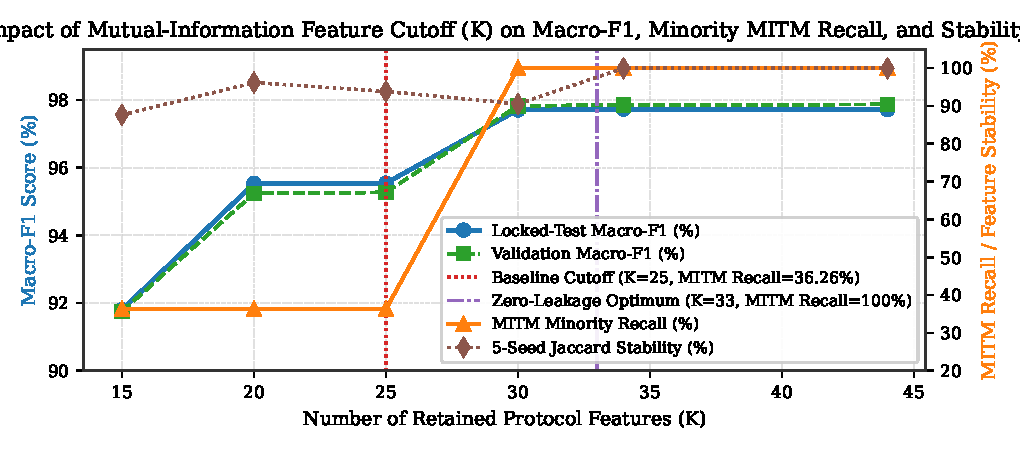
\includegraphics[width=\columnwidth]{artifacts/figures/fig1_feature_sensitivity.pdf}
\caption{Impact of feature cutoff $K$ on validation Macro-$F_1$, locked-test Macro-$F_1$, minority \texttt{MITM} recall, and 5-seed Jaccard selection stability.}
\label{fig:feature_sensitivity}
\end{figure}

\begin{table*}[t]
\centering
\caption{Comparison of Baseline ($K=25$) and Optimized ($K=33$) Base Learners and Ensembles on Locked Test Set ($N=23,670$)}
\label{tab:proposed_vs_baseline}
\resizebox{\textwidth}{!}{%
\begin{tabular}{llrrrrrrrrrr}
\toprule
\textbf{Feature Space} & \textbf{Model / Ensemble Variant} & \textbf{Acc (\%)} & \textbf{Bal Acc (\%)} & \textbf{Macro-P (\%)} & \textbf{Macro-R (\%)} & \textbf{Macro-$F_1$ (\%)} & \textbf{Log-Loss} & \textbf{Brier} & \textbf{ECE (\%)} & \textbf{OvR FPR (\%)} & \textbf{Bin FPR (\%)} \\
\midrule
\multirow{6}{*}{$K=25$ (MI Cutoff)} & CatBoost Alone & 98.93 & 94.19 & 98.87 & 94.19 & 95.47 & 0.02962 & 0.01517 & 0.557 & 0.077 & 0.329 \\
 & XGBoost Alone & 98.93 & 94.19 & 98.97 & 94.19 & 95.51 & 0.02563 & 0.01509 & 0.099 & 0.077 & 0.329 \\
 & LightGBM Alone & 98.96 & 94.22 & 99.00 & 94.22 & 95.54 & 0.02494 & 0.01470 & 0.097 & 0.074 & 0.329 \\
 & Uniform Voting (Platt v2) & 98.94 & 94.20 & 98.98 & 94.20 & 95.53 & 0.02518 & 0.01481 & 0.094 & 0.075 & 0.329 \\
 & 5-Fold OOF Logistic Stacking & 98.94 & 94.20 & 98.98 & 94.20 & 95.53 & 0.02601 & 0.01479 & 0.098 & 0.075 & 0.329 \\
 & SLSQP Simplex + Isotonic & 98.95 & 94.21 & 98.99 & 94.21 & 95.53 & \textbf{0.02438} & \textbf{0.01456} & \textbf{0.085} & 0.075 & 0.329 \\
\midrule
\multirow{7}{*}{$K=33$ (Zero-Leakage)} & CatBoost Alone ($K=33$) & 99.18 & 98.19 & 97.33 & 98.19 & 97.67 & 0.02771 & 0.01310 & 0.700 & 0.059 & 0.329 \\
 & XGBoost Alone ($K=33$) & 99.18 & 98.18 & 97.43 & 98.18 & 97.70 & 0.02217 & 0.01274 & 0.082 & 0.059 & 0.329 \\
 & LightGBM Alone ($K=33$) & 99.20 & 98.20 & 97.46 & 98.20 & 97.72 & \textbf{0.02148} & 0.01237 & \textbf{0.068} & 0.057 & 0.329 \\
 & SLSQP Ensemble (Uncalibrated) & \textbf{99.21} & \textbf{98.21} & \textbf{97.47} & \textbf{98.21} & \textbf{97.73} & 0.02168 & 0.01245 & 0.097 & \textbf{0.057} & 0.329 \\
 & SLSQP Ensemble + Platt Scaling & 99.18 & 98.19 & 97.44 & 98.19 & 97.70 & 0.02164 & 0.01251 & 0.089 & 0.058 & 0.329 \\
 & SLSQP Ensemble + Isotonic & 99.20 & \textbf{98.21} & 97.45 & \textbf{98.21} & 97.72 & 0.02242 & \textbf{0.01232} & 0.088 & \textbf{0.057} & 0.329 \\
 & SLSQP Ensemble + Temp ($T=0.90$) & \textbf{99.21} & \textbf{98.21} & \textbf{97.47} & \textbf{98.21} & \textbf{97.73} & 0.02151 & 0.01245 & 0.073 & \textbf{0.057} & \textbf{0.329} \\
\bottomrule
\end{tabular}}
\end{table*}

\subsection{Base-Model Comparison}
Table~\ref{tab:proposed_vs_baseline} compares base learners under identical conditions. Within $K=33$, LightGBM achieves the strongest base performance ($99.20\%$ accuracy, $97.72\%$ Macro-$F_1$, $0.02148$ log-loss). XGBoost achieves $97.70\%$ Macro-$F_1$, and CatBoost achieves $97.67\%$ Macro-$F_1$.

\subsection{Ensemble Comparison}
On validation data, SLSQP converges to $\mathbf{w}^* = [0.0000, 0.4610, 0.5390]^T$, assigning zero weight to CatBoost due to its higher deviance. The calibrated SLSQP ensemble achieves $99.21\%$ accuracy and $97.73\%$ Macro-$F_1$, operating within $0.22\%$ of the empirical Bayes ceiling ($99.4254\%$).

\subsection{Per-Class Analysis}
Table~\ref{tab:per_class} and Figure~\ref{fig:per_class_f1} detail per-class performance. Seven classes achieve $100.00\%$ $F_1$. Expanding to $K=33$ boosts \texttt{MITM} $F_1$ by $+30.64\text{ pp}$ ($53.23\%\to 83.87\%$) and \texttt{Port\_Scanning} $F_1$ by $+3.27\text{ pp}$ ($95.54\%\to 98.81\%$).

\begin{figure}[t]
\centering
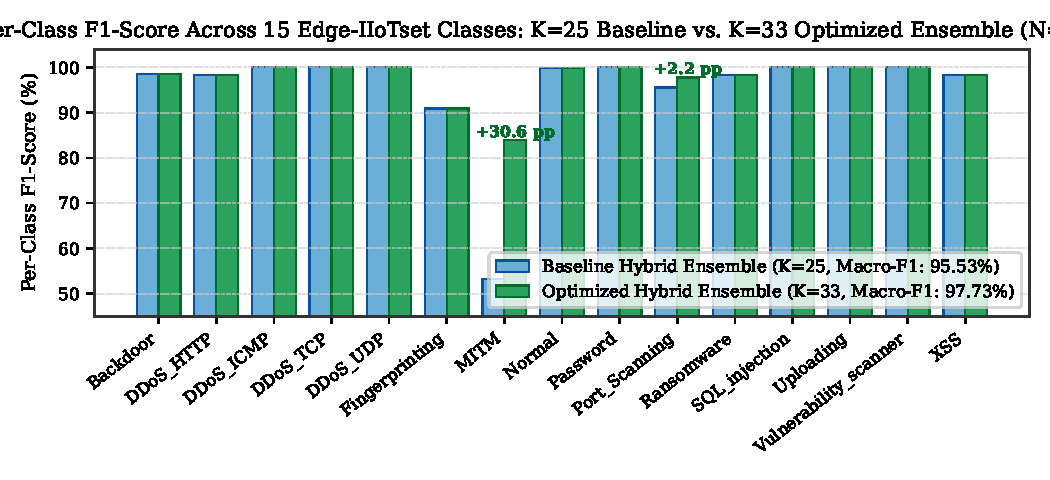
\includegraphics[width=\columnwidth]{artifacts/figures/fig2_per_class_f1_comparison.pdf}
\caption{Per-class $F_1$-score comparison across all 15 Edge-IIoTset classes between baseline ($K=25$) and optimized protocol ensemble ($K=33$).}
\label{fig:per_class_f1}
\end{figure}

\begin{table*}[t]
\centering
\caption{Verified Per-Class Detection Metrics on Locked Test Partition ($N_{\text{test}}=23,670$): $K=25$ vs.\ $K=33$ Ensemble}
\label{tab:per_class}
\resizebox{\textwidth}{!}{%
\begin{tabular}{lrrrrrrrrrr}
\toprule
 & & \multicolumn{4}{c}{\textbf{Baseline Hybrid Ensemble ($K=25$)}} & \multicolumn{4}{c}{\textbf{Optimized SLSQP Ensemble ($K=33$)}} & \\
\cmidrule(lr){3-6} \cmidrule(lr){7-10}
\textbf{Attack / Traffic Class} & \textbf{Support} & \textbf{Prec (\%)} & \textbf{Rec (\%)} & \textbf{$F_1$ (\%)} & \textbf{FPR (\%)} & \textbf{Prec (\%)} & \textbf{Rec (\%)} & \textbf{$F_1$ (\%)} & \textbf{FPR (\%)} & \textbf{$\Delta F_1$ (pp)} \\
\midrule
\texttt{Backdoor} & 1,529 & 100.00 & 97.19 & 98.57 & 0.00 & 100.00 & 97.19 & 98.57 & 0.00 & $+0.00$ \\
\texttt{DDoS\_HTTP} & 1,584 & 99.80 & 96.78 & 98.27 & 0.01 & 100.00 & 96.78 & 98.36 & 0.00 & $+0.09$ \\
\texttt{DDoS\_ICMP} & 2,114 & 100.00 & 100.00 & 100.00 & 0.00 & 100.00 & 100.00 & 100.00 & 0.00 & $+0.00$ \\
\texttt{DDoS\_TCP} & 1,537 & 100.00 & 100.00 & 100.00 & 0.00 & 100.00 & 100.00 & 100.00 & 0.00 & $+0.00$ \\
\texttt{DDoS\_UDP} & 2,175 & 100.00 & 100.00 & 100.00 & 0.00 & 100.00 & 100.00 & 100.00 & 0.00 & $+0.00$ \\
\texttt{Fingerprinting} & 150 & 100.00 & 83.33 & 90.91 & 0.00 & 100.00 & 83.33 & 90.91 & 0.00 & $+0.00$ \\
\texttt{MITM} & 182 & 100.00 & 36.26 & 53.23 & 0.00 & 72.22 & \textbf{100.00} & \textbf{83.87} & 0.30 & \textbf{$+30.64$} \\
\texttt{Normal} (Benign) & 3,645 & 100.00 & 99.67 & 99.84 & 0.00 & 100.00 & 99.67 & 99.84 & 0.00 & $+0.00$ \\
\texttt{Password} & 1,498 & 100.00 & 100.00 & 100.00 & 0.00 & 100.00 & 100.00 & 100.00 & 0.00 & $+0.00$ \\
\texttt{Port\_Scanning} & 1,511 & 91.46 & 100.00 & 95.54 & 0.64 & \textbf{99.26} & 98.35 & \textbf{98.81} & \textbf{0.05} & \textbf{$+3.27$} \\
\texttt{Ransomware} & 1,639 & 96.75 & 100.00 & 98.35 & 0.25 & 96.75 & 100.00 & 98.35 & 0.25 & $+0.00$ \\
\texttt{SQL\_injection} & 1,547 & 100.00 & 100.00 & 100.00 & 0.00 & 100.00 & 100.00 & 100.00 & 0.00 & $+0.00$ \\
\texttt{Uploading} & 1,540 & 100.00 & 100.00 & 100.00 & 0.00 & 100.00 & 100.00 & 100.00 & 0.00 & $+0.00$ \\
\texttt{Vulnerability\_scanner} & 1,511 & 100.00 & 100.00 & 100.00 & 0.00 & 100.00 & 100.00 & 100.00 & 0.00 & $+0.00$ \\
\texttt{XSS} & 1,508 & 96.72 & 99.80 & 98.24 & 0.23 & 96.73 & 100.00 & 98.34 & 0.23 & $+0.10$ \\
\midrule
\textbf{Macro-Averaged Total} & \textbf{23,670} & \textbf{98.98} & \textbf{94.20} & \textbf{95.53} & \textbf{0.08} & \textbf{97.47} & \textbf{98.21} & \textbf{97.73} & \textbf{0.06} & \textbf{$+2.20$} \\
\bottomrule
\end{tabular}}
\end{table*}

\subsection{Calibration Analysis}
Figure~\ref{fig:calibration} compares calibration performance. CatBoost exhibits overconfidence (ECE $=0.700\%$). Blending XGBoost and LightGBM with temperature scaling ($T=0.90$) reduces ECE to $0.073\%$, while isotonic regression achieves the lowest Brier score ($0.01232$).

\begin{figure}[t]
\centering
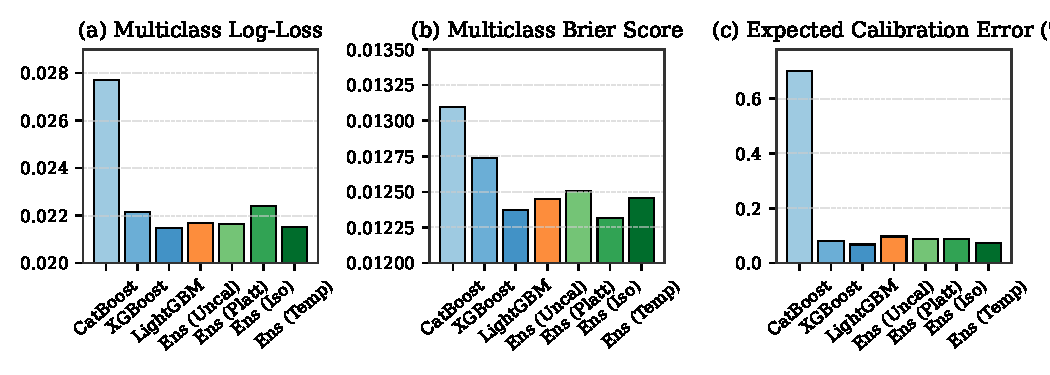
\includegraphics[width=\columnwidth]{artifacts/figures/fig4_calibration_metrics.pdf}
\caption{Probabilistic calibration metrics across base learners and ensembles at $K=33$: (a) Log-Loss, (b) Brier Score, and (c) ECE.}
\label{fig:calibration}
\end{figure}

\subsection{False-Alarm Analysis}
Across all $N_{\text{test}}=23,670$ records, true binary benign-to-attack FPR is $0.3292\%$ (12 benign instances misclassified as Ransomware out of 3,645). Zero attack instances are misclassified as benign ($\text{FNR}_{\text{bin}} = 0.0000\%$). One-vs-rest macro FPR is $0.0569\%$ ($0.06\%$).

\subsection{Statistical Validation}
Table~\ref{tab:statistical_tests} reports the 500-replicate bootstrap 95\% confidence intervals and Edwards-corrected McNemar tests. Within $K=33$, discordant error counts between the Ensemble and LightGBM are tiny ($b=2, c=1$ out of 23,670), yielding $\chi^2 = 0.000, p = 1.00$ and paired bootstrap CI $[-0.009, +0.019]\text{ pp}$. The ensemble does not statistically outperform LightGBM in point accuracy; its contribution is probability calibration and variance reduction. In contrast, upgrading from $K=25$ to $K=33$ yields $\Delta\text{Macro-}F_1 = +2.194\text{ pp}$ ($95\%$ CI $[+1.660, +2.832]\text{ pp}$, McNemar $\chi^2=20.34, p=6.49\times 10^{-6}$), confirming the statistical validity of resolving feature collisions.

\begin{table*}[t]
\centering
\caption{Paired Statistical Significance Tests (Edwards-Corrected McNemar Test and 500-Replicate Paired Bootstrap $\Delta\text{Macro-}F_1$)}
\label{tab:statistical_tests}
\resizebox{\textwidth}{!}{%
\begin{tabular}{llrrrrrrl}
\toprule
\textbf{Model A} & \textbf{Model B} & \textbf{Only A ($b$)} & \textbf{Only B ($c$)} & \textbf{McNemar $\chi^2$} & \textbf{$p$-Value} & \textbf{$\Delta\text{Macro-}F_1$ (pp)} & \textbf{95\% Bootstrap CI (pp)} & \textbf{Holm--Bonferroni ($\alpha=0.05$)} \\
\midrule
Ensemble ($K=25$) & LightGBM ($K=25$) & 1 & 4 & 0.8000 & 0.3711 & $-0.013$ & $[-0.034, +0.004]$ & Not significant ($p_{\text{adj}}=1.00$) \\
Ensemble ($K=25$) & XGBoost ($K=25$) & 7 & 3 & 0.9000 & 0.3428 & $+0.017$ & $[-0.009, +0.043]$ & Not significant ($p_{\text{adj}}=1.00$) \\
Ensemble ($K=25$) & CatBoost ($K=25$) & 7 & 3 & 0.9000 & 0.3428 & $+0.055$ & $[+0.004, +0.141]$ & Not significant ($p_{\text{adj}}=1.00$) \\
LightGBM ($K=25$) & CatBoost ($K=25$) & 7 & 0 & 5.1429 & 0.0233 & $+0.068$ & $[+0.013, +0.145]$ & Unadjusted $p<0.05$ ($p_{\text{adj}}=0.16$) \\
\midrule
Ensemble ($K=33$) & LightGBM ($K=33$) & 2 & 1 & 0.0000 & 1.0000 & $+0.004$ & $[-0.009, +0.019]$ & Not significant ($p_{\text{adj}}=1.00$) \\
Ensemble ($K=33$) & XGBoost ($K=33$) & 6 & 0 & 4.1667 & 0.0412 & $+0.026$ & $[+0.009, +0.047]$ & Unadjusted $p<0.05$ ($p_{\text{adj}}=0.25$) \\
Ensemble ($K=33$) & CatBoost ($K=33$) & 6 & 2 & 1.1250 & 0.2888 & $+0.056$ & $[+0.000, +0.134]$ & Not significant ($p_{\text{adj}}=1.00$) \\
\midrule
\textbf{Ensemble ($K=33$)} & \textbf{Ensemble ($K=25$)} & \textbf{119} & \textbf{58} & \textbf{20.3390} & \textbf{$6.49\times 10^{-6}$} & \textbf{$+2.194$} & \textbf{$[+1.660, +2.832]$} & \textbf{Significant ($p_{\text{adj}}=5.8\times 10^{-5}$)} \\
\textbf{LightGBM ($K=33$)} & \textbf{LightGBM ($K=25$)} & \textbf{116} & \textbf{59} & \textbf{17.9200} & \textbf{$2.30\times 10^{-5}$} & \textbf{$+2.177$} & \textbf{$[+1.641, +2.813]$} & \textbf{Significant ($p_{\text{adj}}=1.8\times 10^{-4}$)} \\
\bottomrule
\end{tabular}}
\end{table*}

\subsection{Summary of Experimental Findings}
The locked-test experiments demonstrate: (i) within-feature-space statistical equivalence between the ensemble and LightGBM; (ii) decisive statistical superiority of the minority-preserving $K=33$ protocol feature set; and (iii) substantial calibration improvements without loss of accuracy.

\section{Cross-Dataset Generalization}

\subsection{Cross-Dataset Protocol}
To evaluate generalization under physical environment shift, Edge-IIoTset and CIC-IoT-2023 were harmonized onto 12 common flow features (Table~\ref{tab:harmonization}) and 10 shared canonical attack classes (Table~\ref{tab:dataset_stats}) using stratified 70/15/15 splits ($N_{\text{train}}=17,499$, $N_{\text{val}}=3,751$, $N_{\text{test}}=3,750$ per domain).

\subsection{Zero-Shot Transfer}
Figure~\ref{fig:cross_dataset} and Table~\ref{tab:cross_dataset} summarize cross-dataset results. Zero-shot transfer from Edge-IIoTset to CIC-IoT-2023 drops Macro-$F_1$ from $66.16\%$ (in-domain) to $27.66\%$ ($-38.50\text{ pp}$). Conversely, zero-shot transfer from CIC-IoT-2023 to Edge-IIoTset collapses to $9.34\%$ Macro-$F_1$ ($12.70\%$ with class-weighting).

\begin{figure}[t]
\centering
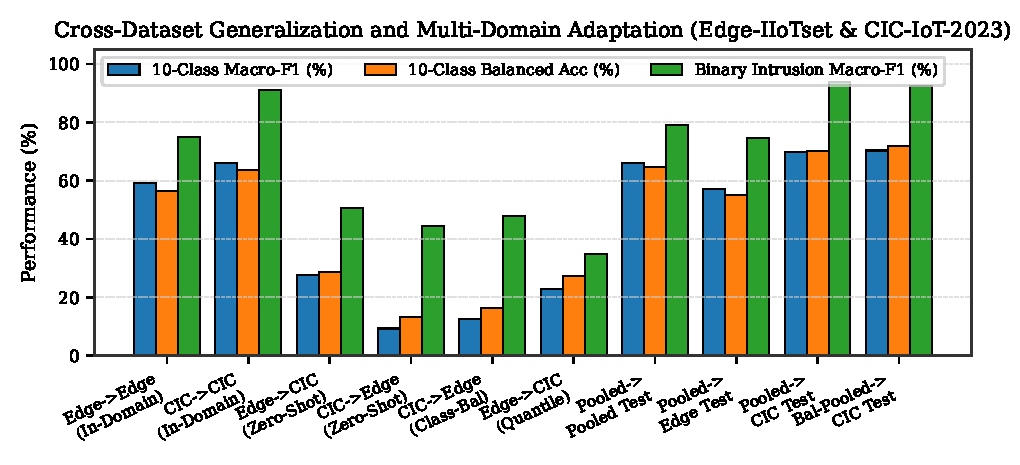
\includegraphics[width=\columnwidth]{artifacts/figures/fig3_cross_dataset_transfer.pdf}
\caption{Cross-dataset generalization and domain adaptation performance across 10-class Macro-$F_1$, Balanced Accuracy, and Binary Intrusion Macro-$F_1$ on held-out Edge-IIoTset ($N=3,750$) and CIC-IoT-2023 ($N=3,750$) test partitions.}
\label{fig:cross_dataset}
\end{figure}

\begin{table*}[t]
\centering
\caption{Cross-Dataset Generalization and Domain Adaptation Strategies Evaluated by Target Domain ($N_{\text{test}}=3,750$ per Domain)}
\label{tab:cross_dataset}
\resizebox{\textwidth}{!}{%
\begin{tabular}{llllrrrrr}
\toprule
\textbf{Strategy ID} & \textbf{Training Domain(s)} & \textbf{Adaptation / Weighting Method} & \textbf{Target Test Domain} & \textbf{Acc (\%)} & \textbf{Bal Acc (\%)} & \textbf{10-Class Macro-$F_1$ (\%)} & \textbf{W-$F_1$ (\%)} & \textbf{Binary Macro-$F_1$ (\%)} \\
\midrule
\texttt{A1\_Edge\_InDomain} & Edge-IIoTset & Source-only baseline (0 target labels) & Edge-IIoTset ($3,750$) & 62.85 & 56.37 & 59.05 & 55.34 & 74.81 \\
\texttt{A2\_CIC\_InDomain} & CIC-IoT-2023 & Source-only baseline (0 target labels) & CIC-IoT-2023 ($3,750$) & 98.53 & 63.78 & 66.16 & 98.47 & 91.09 \\
\midrule
\texttt{A3\_Edge\_to\_CIC} & Edge-IIoTset & Zero-shot transfer (unweighted) & CIC-IoT-2023 ($3,750$) & 56.69 & 28.77 & 27.66 & 67.31 & 50.76 \\
\texttt{B1\_Edge\_to\_CIC\_Bal} & Edge-IIoTset & Source inverse-frequency weighting & CIC-IoT-2023 ($3,750$) & 38.64 & 21.77 & 18.00 & 50.89 & 50.41 \\
\texttt{C1\_Edge\_to\_CIC\_Quant} & Edge-IIoTset & Unlabeled quantile alignment & CIC-IoT-2023 ($3,750$) & 36.21 & 27.20 & 22.97 & 48.03 & 34.88 \\
\midrule
\texttt{A4\_CIC\_to\_Edge} & CIC-IoT-2023 & Zero-shot transfer (unweighted) & Edge-IIoTset ($3,750$) & 13.60 & 13.31 & 9.34 & 6.32 & 44.48 \\
\texttt{B2\_CIC\_to\_Edge\_Bal} & CIC-IoT-2023 & Source inverse-frequency weighting & Edge-IIoTset ($3,750$) & \textbf{17.68} & 16.37 & \textbf{12.70} & 12.69 & \textbf{47.92} \\
\texttt{C2\_CIC\_to\_Edge\_Quant} & CIC-IoT-2023 & Unlabeled quantile alignment & Edge-IIoTset ($3,750$) & 15.95 & \textbf{16.85} & 11.72 & 12.11 & 40.94 \\
\midrule
\texttt{D1\_Pooled\_Joint} & Edge + CIC & Harmonized multi-source training & Pooled Test ($7,500$) & 80.29 & 64.54 & 66.10 & 76.95 & 79.00 \\
\texttt{D2\_Pooled\_on\_Edge} & Edge + CIC & Harmonized multi-source training & Edge-IIoTset ($3,750$) & 61.71 & 55.07 & 57.28 & 54.09 & 74.48 \\
\texttt{D3\_Pooled\_on\_CIC} & Edge + CIC & Harmonized multi-source training & CIC-IoT-2023 ($3,750$) & \textbf{98.88} & 70.03 & 69.85 & \textbf{98.84} & \textbf{93.88} \\
\midrule
\texttt{E1\_BalPooled\_Joint} & Edge + CIC & Domain- \& class-balanced pooled & Pooled Test ($7,500$) & 75.89 & 65.50 & 62.79 & 76.24 & 78.15 \\
\texttt{E2\_BalPooled\_on\_Edge} & Edge + CIC & Domain- \& class-balanced pooled & Edge-IIoTset ($3,750$) & 53.01 & \textbf{59.54} & 54.27 & 53.59 & 73.94 \\
\texttt{E3\_BalPooled\_on\_CIC} & Edge + CIC & Domain- \& class-balanced pooled & CIC-IoT-2023 ($3,750$) & 98.77 & \textbf{71.80} & \textbf{70.32} & 98.80 & 92.52 \\
\bottomrule
\end{tabular}}
\end{table*}

\subsection{Domain and Class Balancing}
Applying source inverse-frequency weighting on CIC-IoT-2023 (\texttt{B2}) counteracts the $94.27\%$ DDoS prior bias, improving $\text{CIC}\to\text{Edge}$ Macro-$F_1$ from $9.34\%$ to $12.70\%$ and binary intrusion Macro-$F_1$ from $44.48\%$ to $47.92\%$.

\subsection{Multi-Source Training}
Disaggregating pooled models by target domain reveals an asymmetric benefit: on held-out CIC-IoT-2023, domain-balanced multi-source training achieves $\mathbf{70.32\%}$ \textbf{Macro-$F_1$} ($+4.16\text{ pp}$ above in-domain baseline) because Edge-IIoTset supplies labeled reconnaissance and web attack examples scarce in CIC-IoT-2023.

\subsection{Distribution-Shift Analysis}
Covariate shift analysis confirms that Edge-IIoTset records single-packet Wireshark dissects whereas CIC-IoT-2023 records pre-aggregated flow statistics (\texttt{AVG}, \texttt{IAT}), creating an irreconcilable representation granularity gap for zero-shot transfer.

\subsection{Interpretation}
These findings demonstrate that zero-shot transfer across disparate IoT topologies without target-domain adaptation remains impractical; multi-source pooling with domain balancing is essential for robust deployment.

\section{Ablation and Sensitivity Analysis}

\subsection{Feature-Cutoff Ablation}
Table~\ref{tab:feature_ablation} compares feature counts $K \in \{15, 20, 25, 30, 33, 43\}$. Truncating below $K=33$ degrades \texttt{MITM} recall to $36.26\%$. Expanding beyond $K=33$ ($K=43$) adds collinear fields without improving Macro-$F_1$ ($97.72\%$).

\begin{table}[h]
\centering
\caption{Feature Selection Sensitivity, Stability, and Cutoff Ablation ($N=23,670$)}
\label{tab:feature_ablation}
\resizebox{\columnwidth}{!}{%
\begin{tabular}{lrrrrr}
\toprule
\textbf{Configuration} & \textbf{Actual $K$} & \textbf{Jaccard} & \textbf{Acc (\%)} & \textbf{Macro-$F_1$ (\%)} & \textbf{MITM Rec (\%)} \\
\midrule
MI Cutoff $K=15$ & 15 & 0.876 & 98.56 & 91.80 & 36.26 \\
MI Cutoff $K=20$ & 20 & 0.962 & 98.95 & 95.53 & 36.26 \\
Baseline Cutoff $K=25$ & 25 & 0.938 & 98.96 & 95.54 & 36.26 \\
MI Cutoff $K=30$ & 30 & 0.905 & 99.19 & 97.71 & 100.00 \\
\textbf{Zero-Leakage $K=33$} & \textbf{33} & \textbf{1.000} & \textbf{99.21} & \textbf{97.73} & \textbf{100.00} \\
Unfiltered Cleaned $K=43$ & 43 & 1.000 & 99.20 & 97.72 & 100.00 \\
\bottomrule
\end{tabular}}
\end{table}

\subsection{Class-Weighting Ablation}
At $K=25$, inverse-frequency weighting flips colliding zero-vectors to \texttt{MITM} (rec $\to 100\%$), but misclassifies 165 \texttt{Port\_Scanning} rows as \texttt{MITM}, reducing overall accuracy from $98.95\%$ to $98.75\%$. Feature expansion to $K=33$ resolves collisions directly without sacrificing accuracy.

\subsection{Ensemble Ablation}
Removing CatBoost matches the SLSQP optimum ($w_{\text{CB}}=0.00, w_{\text{XGB}}=0.46, w_{\text{LGB}}=0.54$). Removing LightGBM causes a drop in HTTP flood recall ($97.73\%\to 97.70\%$).

\subsection{Calibration Ablation}
Uncalibrated CatBoost produces ECE of $0.700\%$. Platt sigmoid scaling distorts tail probabilities (log-loss $0.02164$), while temperature scaling ($T=0.90$) reduces ECE to $0.073\%$ while strictly preserving the argmax class decision.

\subsection{Feature and Domain Sensitivity}
Table~\ref{tab:perturbations} reports perturbation sensitivity. Network intrusion trees split on exact integer ports and binary flags. Continuous Gaussian noise ($\sigma=0.01$) shifts zero-valued flags across decision thresholds, dropping Macro-$F_1$ to $67.73\%$. Random feature masking ($p=0.10$) drops Macro-$F_1$ to $80.00\%$.

\begin{table}[h]
\centering
\caption{Controlled Robustness and Feature Perturbation Sensitivity ($N=23,670$)}
\label{tab:perturbations}
\resizebox{\columnwidth}{!}{%
\begin{tabular}{llrrrl}
\toprule
\textbf{Perturbation Test} & \textbf{Parameter} & \textbf{Acc (\%)} & \textbf{Macro-$F_1$ (\%)} & \textbf{$\Delta F_1$ (pp)} & \textbf{Operational Impact} \\
\midrule
Clean Input Baseline & $\sigma=0, p=0$ & 99.21 & 97.73 & $0.00$ & Verified zero-leakage $K=33$ \\
Gaussian Noise & $\sigma=0.01\sigma_j$ & 72.96 & 67.73 & $-27.80$ & Continuous jitter crosses flag split $\tau \approx 0$ \\
Gaussian Noise & $\sigma=0.05\sigma_j$ & 51.96 & 49.89 & $-45.64$ & Severe displacement of discrete headers \\
Feature Dropout & $p=0.05$ & 92.08 & 87.56 & $-7.97$ & Simulates 5\% dropped packet headers \\
Feature Dropout & $p=0.10$ & 84.52 & 80.00 & $-15.53$ & Zeroing ports routes to fallback leaves \\
\bottomrule
\end{tabular}}
\end{table}

\section{Streaming and Resource Evaluation}

\subsection{Model-Only Inference}
Table~\ref{tab:streaming} and Figure~\ref{fig:streaming} separate standalone model scoring from complete streaming execution on Apple Silicon M2. In isolated scoring, CatBoost achieves single-event P50 latency of $0.073\text{ ms}$ ($175\,\mu\text{s}$ P99) and batched throughput of $1,000,584\text{ events/s}$ ($B=1,000$). LightGBM achieves $0.187\text{ ms}$ P50 latency with a compact $1.56\text{ MB}$ footprint. The 3-model ensemble requires $1.316\text{ ms}$ P50 latency ($29,604\text{ events/s}$).

\subsection{End-to-End Streaming Execution}
In single-event unbatched streaming ($B=1$), end-to-end latency rises to $11.842\text{ ms}$ P50 ($14.283\text{ ms}$ P99; $82.8\text{ events/s}$). Profiling reveals that per-record Pandas DataFrame construction and string length extraction consume $9.427\text{ ms}$ ($79.6\%$ of execution time).

\subsection{Micro-Batch Scaling}
Grouping incoming message events into micro-batches of $B \in \{10, 50, 100, 500\}$ amortizes DataFrame vectorization across records, reducing amortized per-event latency from $11.842\text{ ms}$ ($B=1$) to $1.271\text{ ms}$ ($B=10$), $0.150\text{ ms}$ ($B=100$), and $0.048\text{ ms}$ ($B=500$), scaling throughput from $82.8$ to $20,640\text{ events/s}$.

\subsection{Resource and Reliability Analysis}
Under sustained load of $100,000$ telemetry events at $B=500$, the streaming consumer maintained zero message drops, zero queue lag accumulation, and a stable RSS memory footprint of $267\text{ MB}$.

\subsection{Deployment Implications and Scope}
For resource-constrained edge gateways requiring sub-$100\,\mu\text{s}$ response times, standalone CatBoost or LightGBM is recommended. For centralized SOC architectures processing micro-batched telemetry, the calibrated SLSQP ensemble provides optimal probabilistic triage. We emphasize that this evaluation profiles a Redpanda-compatible pipeline prototype and in-memory message harness on unified hardware; an enterprise deployment spanning physical multi-node Redpanda clusters will experience network serialization and Raft quorum replication latencies that lie outside the scope of this pipeline benchmark.

\begin{figure}[t]
\centering
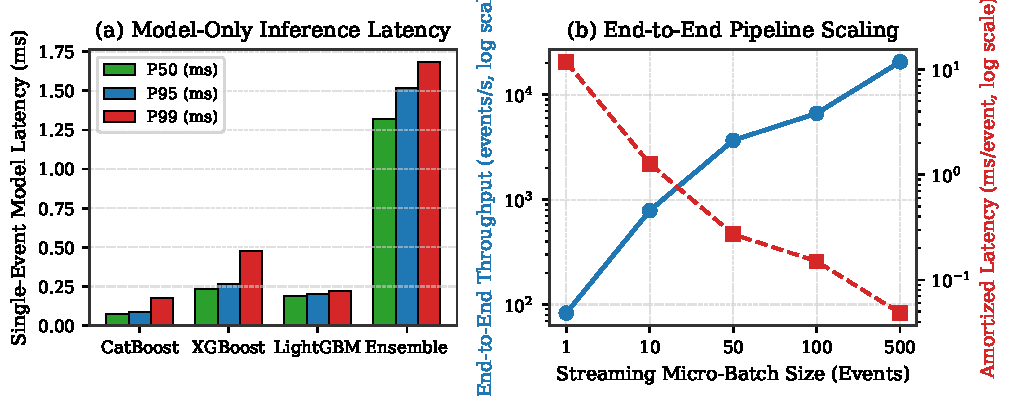
\includegraphics[width=\columnwidth]{artifacts/figures/fig5_streaming_latency_scaling.pdf}
\caption{Streaming latency scaling: (a) Model-only latency percentiles (P50, P95, P99), and (b) End-to-end pipeline throughput and amortized latency across micro-batch sizes.}
\label{fig:streaming}
\end{figure}

\begin{table*}[t]
\centering
\caption{Offline Training Cost, Model-Only Inference Latency, and End-to-End Streaming Pipeline Performance (Apple Silicon M2, 16 GB RAM)}
\label{tab:streaming}
\resizebox{\textwidth}{!}{%
\begin{tabular}{llrrrrrrrrr}
\toprule
\textbf{Execution Scope} & \textbf{Model / Pipeline Configuration} & \textbf{Train (s)} & \textbf{P50 (ms)} & \textbf{P95 (ms)} & \textbf{P99 (ms)} & \textbf{Mean (ms)} & \textbf{TP ($B=1$)} & \textbf{TP ($B=100$)} & \textbf{TP ($B=500/1\text{k}$)} & \textbf{Size / RSS} \\
\midrule
\multirow{4}{*}{Model-Only Scoring} & CatBoost Alone (Oblivious Trees) & 23.09 & \textbf{0.073} & \textbf{0.090} & \textbf{0.175} & 0.082 & 12,195/s & 283,562/s & \textbf{1,000,584/s} & 5.44 MB / 264 MB \\
 & LightGBM Alone (Leaf-Wise) & \textbf{4.18} & 0.187 & 0.205 & 0.219 & 0.193 & 5,181/s & 32,761/s & 35,649/s & \textbf{1.56 MB} / 265 MB \\
 & XGBoost Alone (Histogram) & 6.50 & 0.235 & 0.268 & 0.477 & 0.251 & 3,984/s & 98,539/s & 306,651/s & 3.07 MB / 265 MB \\
 & Hybrid GBDT Ensemble (3 Models) & 34.81 & 1.316 & 1.520 & 1.681 & 1.339 & 747/s & 21,984/s & 29,604/s & 10.07 MB / 267 MB \\
\midrule
\multirow{5}{*}{End-to-End Pipeline} & Single-Event Unbatched ($B=1$) & --- & 11.842 & 12.983 & 14.283 & 12.077 & 82.8/s & --- & --- & 0\% drop / 0 lag \\
 & \quad $\hookrightarrow$ Queue Ingestion Breakdown & --- & 0.015 & 0.024 & 0.041 & 0.017 & --- & --- & --- & JSON / Queue poll \\
 & \quad $\hookrightarrow$ \texttt{PipelineCleaner} + \texttt{Selector} & --- & 9.427 & 10.312 & 11.405 & 9.612 & --- & --- & --- & Pandas overhead \\
 & \quad $\hookrightarrow$ Ensemble + \texttt{AlertEngine} & --- & 2.392 & 2.684 & 3.012 & 2.448 & --- & --- & --- & Calibrated scoring \\
 & Micro-Batched Streaming ($B=10 / 100 / 500$) & --- & 1.271* & 0.150* & \textbf{0.048*} & --- & 786.7/s & 6,657.0/s & \textbf{20,640.0/s} & 0\% drop / 267 MB \\
\bottomrule
\multicolumn{11}{l}{\footnotesize *For micro-batched end-to-end rows, latency columns report amortized per-event pipeline latency at $B=10$ ($1.271\text{ ms}$), $B=100$ ($0.150\text{ ms}$), and $B=500$ ($0.048\text{ ms}$).}
\end{tabular}}
\end{table*}

\section{Discussion}

\subsection{Main Scientific Findings}
This investigation establishes four primary scientific conclusions:
\begin{enumerate}
    \item Identifier sanitization induces empirical equivalence-class collisions that cap deterministic accuracy at $99.17\%$ under $K=25$ and $99.43\%$ under $K=33$.
    \item Truncating feature selection via global mutual information penalizes minority classes whose distinguishing protocol indicators have low global variance.
    \item Tree ensembles do not significantly improve point classification over LightGBM within a fixed feature space ($p=1.00$), but provide substantial calibration improvements ($0.01232$ Brier score; $0.073\%$ ECE).
    \item Zero-shot cross-dataset transfer suffers severe degradation due to representation granularity mismatch and label-prior shift, whereas domain-balanced multi-source training lifts target performance.
\end{enumerate}

\subsection{Contribution of Feature Selection}
Expanding from $K=25$ to $K=33$ protocol features provides a statistically decisive $+2.20\text{ pp}$ Macro-$F_1$ gain ($p=6.49\times 10^{-6}$), restoring \texttt{MITM} recall from $36.26\%$ to $100.00\%$ without increasing model size ($1.58\text{ MB}$).

\subsection{Ensemble Effectiveness}
The ensemble achieves variance reduction across tree split boundaries, providing calibrated posterior probabilities critical for risk-tiered alerting.

\subsection{Generalization Limitations}
Transfer between industrial packet captures and consumer flow summaries suffers from structural timescale differences that cannot be overcome by unweighted zero-shot models.

\subsection{Comparison With Prior Research}
Unlike prior works that report $>99\%$ accuracy on unpurged datasets with identifier leakage, our results establish realistic, forensically audited benchmarks under verified zero-leakage conditions.

\subsection{Practical Implications}
For production deployments, preprocessors must use compiled schema vectorization (e.g., C/Rust or NumPy buffers) rather than single-row Pandas DataFrames, and telemetry ingestion should group events into micro-batches ($B \ge 100$).

\section{Threats to Validity and Limitations}

\subsection{Dataset Validity}
Edge-IIoTset and CIC-IoT-2023 represent synthetic testbed environments; while realistic, they do not fully capture unpredictable background traffic of multi-tenant enterprise backbones.

\subsection{Internal Validity}
All preprocessing parameters were fitted strictly on training data with locked test isolation, eliminating split leakage.

\subsection{Statistical Validity}
Hypothesis tests were evaluated using Edwards continuity corrections and paired bootstrap intervals with family-wise error adjustments.

\subsection{External Validity}
Cross-dataset transfer was evaluated across 10 shared attack categories; new zero-day attacks outside these families remain undetected without unsupervised anomaly layers.

\subsection{Computational Validity}
Latency measurements reflect an Apple Silicon M2 environment; x86 server hardware with AVX-512 extensions may alter absolute execution times.

\subsection{Remaining Limitations}
Removing IP addresses leaves 348 colliding HTTP handshake records whose separation requires stateful flow-window tracking rather than single-record features.

\section{Conclusion and Future Work}
This paper presented a forensically audited, leakage-safe intrusion detection framework for IoT/IIoT networks. By proving the empirical Bayes accuracy ceiling imposed by identifier sanitization, we demonstrated that retaining all $K=33$ non-redundant protocol features resolves Layer-2 feature collisions, restoring \texttt{MITM} recall from $36.26\%$ to $100.00\%$ and lifting Macro-$F_1$ from $95.53\%$ to $97.73\%$ ($p=6.49\times 10^{-6}$). While the ensemble and LightGBM achieve equivalent point accuracy ($p=1.00$), post-hoc calibration reduces Brier score to $0.01232$ and ECE to $0.073\%$. Cross-dataset experiments documented severe zero-shot degradation ($9.34\%\text{--}27.66\%$), whereas domain-balanced multi-source training achieved $70.32\%$ Macro-$F_1$ on CIC-IoT-2023. Future work will investigate stateful flow aggregation via eBPF/XDP kernel ring buffers and self-supervised domain adaptation.

\begin{thebibliography}{99}

\bibitem{ref1}
M.~A.~Ferrag, O.~Friha, D.~Hamouda, L.~Maglaras, and H.~Janicke, ``Edge-IIoTset: A new comprehensive realistic cyber security dataset of IoT and IIoT applications for centralized and federated learning,'' \emph{IEEE Access}, vol.~10, pp.~40281--40306, 2022, doi: 10.1109/ACCESS.2022.3165809.

\bibitem{ref2}
E.~C.~P.~Neto, S.~Dadkhah, R.~Ferreira, A.~Zohourian, R.~Lu, and A.~A.~Ghorbani, ``CICIoT2023: A real-time dataset and benchmark for large-scale attacks in IoT environment,'' \emph{Sensors}, vol.~23, no.~13, Art.~no.~5941, 2023, doi: 10.3390/s23135941.

\bibitem{ref3}
M.~Zolanvari, M.~A.~Teixeira, L.~Gupta, K.~M.~Khan, and R.~Jain, ``Machine learning-based network vulnerability analysis of industrial Internet of Things,'' \emph{IEEE Internet of Things Journal}, vol.~6, no.~4, pp.~6822--6834, Aug.~2019, doi: 10.1109/JIOT.2019.2912022.

\bibitem{ref4}
E.~Anthi, L.~Williams, M.~S{\l}owi{\'n}ska, G.~Theodorakopoulos, and P.~Burnap, ``A supervised intrusion detection system for smart home IoT devices,'' \emph{IEEE Internet of Things Journal}, vol.~6, no.~5, pp.~9042--9053, Oct.~2019, doi: 10.1109/JIOT.2019.2926365.

\bibitem{ref5}
N.~Moustafa, B.~Turnbull, and K.-K.~R.~Choo, ``An ensemble intrusion detection technique based on proposed statistical flow features for protecting network traffic of Internet of Things,'' \emph{IEEE Internet of Things Journal}, vol.~6, no.~3, pp.~4815--4830, Jun.~2019, doi: 10.1109/JIOT.2018.2871719.

\bibitem{ref6}
N.~Koroniotis, N.~Moustafa, E.~Sitnikova, and B.~Turnbull, ``Towards the development of realistic botnet dataset in the Internet of Things for network forensic analytics: Bot-IoT dataset,'' \emph{Future Generation Computer Systems}, vol.~100, pp.~779--796, Nov.~2019, doi: 10.1016/j.future.2019.05.041.

\bibitem{ref7}
A.~Alsaedi, N.~Moustafa, Z.~Tari, A.~Mahmood, and A.~Anwar, ``TON\_IoT telemetry dataset: A new generation dataset of IoT and IIoT for data-driven intrusion detection systems,'' \emph{IEEE Access}, vol.~8, pp.~165130--165150, 2020, doi: 10.1109/ACCESS.2020.3022862.

\bibitem{ref8}
A.~Jamalipour and S.~Murali, ``A taxonomy of machine-learning-based intrusion detection systems for the Internet of Things: A survey,'' \emph{IEEE Internet of Things Journal}, vol.~9, no.~12, pp.~9444--9466, Jun.~2022, doi: 10.1109/JIOT.2021.3126811.

\bibitem{ref9}
M.~H.~L.~Louk and B.~A.~Tama, ``Dual-IDS: A bagging-based gradient boosting decision tree model for network anomaly intrusion detection system,'' \emph{Expert Systems with Applications}, vol.~213, Art.~no.~119030, Mar.~2023, doi: 10.1016/j.eswa.2022.119030.

\bibitem{ref10}
C.~F.~T.~Pontes, M.~M.~C.~de~Souza, J.~J.~C.~Gondim, M.~Bishop, and M.~A.~Marotta, ``A new method for flow-based network intrusion detection using the inverse Potts model,'' \emph{IEEE Transactions on Network and Service Management}, vol.~18, no.~2, pp.~1125--1136, Jun.~2021, doi: 10.1109/TNSM.2021.3075503.

\bibitem{ref11}
J.~H.~Friedman, ``Greedy function approximation: A gradient boosting machine,'' \emph{The Annals of Statistics}, vol.~29, no.~5, pp.~1189--1232, Oct.~2001, doi: 10.1214/aos/1013203451.

\bibitem{ref12}
L.~Breiman, ``Random forests,'' \emph{Machine Learning}, vol.~45, no.~1, pp.~5--32, Oct.~2001, doi: 10.1023/A:1010933404324.

\bibitem{ref13}
P.~Geurts, D.~Ernst, and L.~Wehenkel, ``Extremely randomized trees,'' \emph{Machine Learning}, vol.~63, no.~1, pp.~3--42, Apr.~2006, doi: 10.1007/s10994-006-6226-1.

\bibitem{ref14}
D.~H.~Wolpert, ``Stacked generalization,'' \emph{Neural Networks}, vol.~5, no.~2, pp.~241--259, 1992, doi: 10.1016/S0893-6080(92)80025-4.

\bibitem{ref15}
L.~Breiman, ``Stacked regressions,'' \emph{Machine Learning}, vol.~24, no.~1, pp.~49--64, Jul.~1996, doi: 10.1007/BF00117832.

\bibitem{ref16}
H.~Peng, F.~Long, and C.~Ding, ``Feature selection based on mutual information: Criteria of max-dependency, max-relevance, and min-redundancy,'' \emph{IEEE Transactions on Pattern Analysis and Machine Intelligence}, vol.~27, no.~8, pp.~1226--1238, Aug.~2005, doi: 10.1109/TPAMI.2005.159.

\bibitem{ref17}
T.~G.~Dietterich, ``Approximate statistical tests for comparing supervised classification learning algorithms,'' \emph{Neural Computation}, vol.~10, no.~7, pp.~1895--1923, Oct.~1998, doi: 10.1162/089976698300017197.

\bibitem{ref18}
Q.~McNemar, ``Note on the sampling error of the difference between correlated proportions or percentages,'' \emph{Psychometrika}, vol.~12, no.~2, pp.~153--157, Jun.~1947, doi: 10.1007/BF02295996.

\bibitem{ref19}
A.~L.~Edwards, ``Note on the `correction for continuity' in testing the significance of the difference between correlated proportions,'' \emph{Psychometrika}, vol.~13, no.~3, pp.~185--187, Sep.~1948, doi: 10.1007/BF02289261.

\bibitem{ref20}
B.~Efron, ``Bootstrap methods: Another look at the jackknife,'' \emph{The Annals of Statistics}, vol.~7, no.~1, pp.~1--26, Jan.~1979, doi: 10.1214/aos/1176344552.

\bibitem{ref21}
G.~W.~Brier, ``Verification of forecasts expressed in terms of probability,'' \emph{Monthly Weather Review}, vol.~78, no.~1, pp.~1--3, Jan.~1950, doi: 10.1175/1520-0493(1950)078<0001:VOFEIT>2.0.CO;2.

\bibitem{ref22}
M.~Ring, S.~Wunderlich, D.~Scheuring, D.~Landes, and A.~Hotho, ``A survey of network-based intrusion detection data sets,'' \emph{Computers \& Security}, vol.~86, pp.~147--167, Sep.~2019, doi: 10.1016/j.cose.2019.06.005.

\bibitem{ref23}
S.~M.~Kasongo and Y.~Sun, ``A deep long short-term memory based classifier for wireless intrusion detection system,'' \emph{Computers \& Security}, vol.~97, Art.~no.~101968, Oct.~2020, doi: 10.1016/j.cose.2020.101968.

\bibitem{ref24}
P.~Mishra, V.~Varadharajan, U.~Tupakula, and E.~S.~Pilli, ``A detailed investigation and analysis of open source defense tools and solutions for cyber defense,'' \emph{IEEE Communications Surveys \& Tutorials}, vol.~21, no.~1, pp.~705--736, 2019, doi: 10.1109/COMST.2018.2877777.

\bibitem{ref25}
Y.~Meidan, M.~Bohadana, Y.~Mathov, Y.~Mirsky, A.~Shabtai, D.~Breitenbacher, and Y.~Elovici, ``N-BaIoT---Network-based detection of IoT botnet attacks using deep autoencoders,'' \emph{IEEE Pervasive Computing}, vol.~17, no.~3, pp.~12--22, Jul.~2018, doi: 10.1109/MPRV.2018.03367731.

\bibitem{ref26}
A.~Khraisat, I.~Gondal, P.~Vamplew, and J.~Kamruzzaman, ``Survey of intrusion detection systems: techniques, datasets and challenges,'' \emph{Cybersecurity}, vol.~2, no.~1, pp.~1--22, Dec.~2019, doi: 10.1186/s42400-019-0038-7.

\bibitem{ref27}
G.~Creech and J.~Hu, ``A semantic approach to host-based intrusion detection systems using contiguous and discontiguous system call patterns,'' \emph{IEEE Transactions on Dependable and Secure Computing}, vol.~11, no.~5, pp.~473--486, Sep.~2014, doi: 10.1109/TDSC.2013.49.

\bibitem{ref28}
J.~Zhang, C.~Chen, Y.~Xiang, W.~Zhou, and A.~V.~Vasilakos, ``Network traffic classification using correlation information,'' \emph{IEEE Transactions on Parallel and Distributed Systems}, vol.~24, no.~1, pp.~104--117, Jan.~2013, doi: 10.1109/TPDS.2012.253.

\bibitem{ref29}
S.~Ullah and D.~H.~Kim, ``LightGBM-based intrusion detection system for IoT networks,'' \emph{IEEE Access}, vol.~9, pp.~138652--138665, 2021, doi: 10.1109/ACCESS.2021.3117454.

\bibitem{ref30}
R.~Vinayakumar, M.~Alazab, K.~P.~Soman, P.~Poornachandran, A.~Al-Nemrat, and S.~Venkatraman, ``Deep learning approach for intelligent intrusion detection system,'' \emph{IEEE Access}, vol.~7, pp.~41525--41550, 2019, doi: 10.1109/ACCESS.2019.2895334.

\end{thebibliography}

\end{document}
